% Options for packages loaded elsewhere
\PassOptionsToPackage{unicode}{hyperref}
\PassOptionsToPackage{hyphens}{url}
%
\documentclass[
]{article}
\usepackage{lmodern}
\usepackage{amssymb,amsmath}
\usepackage{ifxetex,ifluatex}
\ifnum 0\ifxetex 1\fi\ifluatex 1\fi=0 % if pdftex
  \usepackage[T1]{fontenc}
  \usepackage[utf8]{inputenc}
  \usepackage{textcomp} % provide euro and other symbols
\else % if luatex or xetex
  \usepackage{unicode-math}
  \defaultfontfeatures{Scale=MatchLowercase}
  \defaultfontfeatures[\rmfamily]{Ligatures=TeX,Scale=1}
\fi
% Use upquote if available, for straight quotes in verbatim environments
\IfFileExists{upquote.sty}{\usepackage{upquote}}{}
\IfFileExists{microtype.sty}{% use microtype if available
  \usepackage[]{microtype}
  \UseMicrotypeSet[protrusion]{basicmath} % disable protrusion for tt fonts
}{}
\makeatletter
\@ifundefined{KOMAClassName}{% if non-KOMA class
  \IfFileExists{parskip.sty}{%
    \usepackage{parskip}
  }{% else
    \setlength{\parindent}{0pt}
    \setlength{\parskip}{6pt plus 2pt minus 1pt}}
}{% if KOMA class
  \KOMAoptions{parskip=half}}
\makeatother
\usepackage{xcolor}
\IfFileExists{xurl.sty}{\usepackage{xurl}}{} % add URL line breaks if available
\IfFileExists{bookmark.sty}{\usepackage{bookmark}}{\usepackage{hyperref}}
\hypersetup{
  pdftitle={Effects of bariatric surgery and weight loss on resting state functional connectivity},
  pdfauthor={Hannah Sophie Heinrichs* {[}1{]}; Frauke Beyer* {[}1{]}{[}2{]}; Kristin Prehn; Jürgen Ordemann; Agnes Floel; A. Veronica Witte {[}1{]}{[}2{]}{[}3{]}},
  hidelinks,
  pdfcreator={LaTeX via pandoc}}
\urlstyle{same} % disable monospaced font for URLs
\usepackage[margin=1in]{geometry}
\usepackage{longtable,booktabs}
% Correct order of tables after \paragraph or \subparagraph
\usepackage{etoolbox}
\makeatletter
\patchcmd\longtable{\par}{\if@noskipsec\mbox{}\fi\par}{}{}
\makeatother
% Allow footnotes in longtable head/foot
\IfFileExists{footnotehyper.sty}{\usepackage{footnotehyper}}{\usepackage{footnote}}
\makesavenoteenv{longtable}
\usepackage{graphicx,grffile}
\makeatletter
\def\maxwidth{\ifdim\Gin@nat@width>\linewidth\linewidth\else\Gin@nat@width\fi}
\def\maxheight{\ifdim\Gin@nat@height>\textheight\textheight\else\Gin@nat@height\fi}
\makeatother
% Scale images if necessary, so that they will not overflow the page
% margins by default, and it is still possible to overwrite the defaults
% using explicit options in \includegraphics[width, height, ...]{}
\setkeys{Gin}{width=\maxwidth,height=\maxheight,keepaspectratio}
% Set default figure placement to htbp
\makeatletter
\def\fps@figure{htbp}
\makeatother
\setlength{\emergencystretch}{3em} % prevent overfull lines
\providecommand{\tightlist}{%
  \setlength{\itemsep}{0pt}\setlength{\parskip}{0pt}}
\setcounter{secnumdepth}{5}
\usepackage[left]{lineno}
\linenumbers
\usepackage{subfig}
\usepackage{booktabs}
\usepackage{longtable}
\usepackage{array}
\usepackage{multirow}
\usepackage{wrapfig}
\usepackage{float}
\usepackage{colortbl}
\usepackage{pdflscape}
\usepackage{tabu}
\usepackage{threeparttable}
\usepackage{threeparttablex}
\usepackage[normalem]{ulem}
\usepackage{makecell}
\usepackage{xcolor}

\title{Effects of bariatric surgery and weight loss on resting state functional connectivity}
\author{Hannah Sophie Heinrichs* {[}1{]} \and Frauke Beyer* {[}1{]}{[}2{]} \and Kristin Prehn \and Jürgen Ordemann \and Agnes Floel \and A. Veronica Witte {[}1{]}{[}2{]}{[}3{]}}
\date{1 Max-Planck-Institute for Human Cognitive and Brain Sciences, Leipzig \newline 2 CRC 1052 ``Obesity Mechanisms'', Subproject A1, University of Leipzig \newline 3 Day Clinic for Cognitive Neurology, University Clinic Leipzig}

\begin{document}
\maketitle

{
\setcounter{tocdepth}{2}
\tableofcontents
}
\newpage

\hypertarget{abstract}{%
\section{Abstract}\label{abstract}}

\newpage

\hypertarget{introduction}{%
\section{Introduction}\label{introduction}}

Obesity is a worldwide health issue, enchaining huge personal and societal costs. Excess amount of fat not only affects cardiovascular and metabolic health, but also increases the risk for cognitive decline and dementia later in life.
Conservative treatment options including dietary modification, physical activity and behavioral therapy often do not yield the desired weight loss, especially in patients with very high BMI (\textgreater{} 35 kg/m2). Here, bariatric surgery is a viable option to rapidly induce weight loss and improve glycemic status.
Roux-en-Y gastric bypass (RYGB) is the most effective surgical procedure (Berthoud, Shin, and Zheng", n.d.). Here, a small pouch is formed from the proximal stomach and connected to the jejunum, disconnecting the larger part of the stomach and the proximal part of the small intestine intact from the digestive flow. Other techniques like vertical sleeve gastrectomy (VSG) and gastric banding (GB) reduce stomach volume, but leave the small intestine unchanged (Mulla, Middelbeek, and Patti 2017).
RYGB-induced weight loss is in part mediated by malabsorption of certain nutrients, especially fat, and reduced digestion efficiency (Berthoud, Shin, and Zheng", n.d.) while the role of increased energy expenditure after RYGB is still unclear (Yarmush, D'Alessandro, and Saeidi 2017; Lamarca et al. 2019). Most importantly, RYGB alters the signaling cascades between the gut, fat tissue and the brain and thereby induces profound changes in the regulation of food intake and energy homeostasis (Berthoud, Shin, and Zheng", n.d.). RYBG-patients frequently report altered smell and taste perception, i.e.~increased sensitivity to sweet taste, show less desire to consume high-calorie and high-fat foods and actually reduce intake of such food items (Mulla, Middelbeek, and Patti 2017, @Berthoud\_2011). These changes in appetitive and reward signaling likely relate to altered gut-brain communication, mediated by afferent vagal nerve signaling and gut hormones like GLP-1, PYY and ghrelin (Brutman, Sirohi, and Davis 2019).
Yet, precise mechanisms how bariatric surgery leads to altered appetitive and reward signaling are yet to be elucidated.
Resting state functional magnetic resonance imaging (rsfMRI) is a powerful technique to investigate the dynamic organization of the brain via the correlation of spontaneous neural activity. Anatomically distinct brain regions show functional connectivity (FC), i.e.~correlated neural activity over time, in the absence of a cognitive task. Crucially, these brain networks correspond to networks activated during specific cognitive processes, e.g.~visual, auditory and somatosensory processing, or higher-order cognitive functions, i.e.~attention and executive control (Smith et al. 2009), and can thus be seen as default configuration of the brain. In the context of bariatric surgery, the default mode network, a higher-order network, involved in interoception and governing shifts between external-internal processes, and the reward network, processing hedonic value and internal motivation, are promising candidates to mediate altered gut-brain signaling.
The default mode network has been discovered as a ``task-negative'' network, and is involved in a variety of largely internally-directed cognitive functions including interoception, mind wandering and memory. Its core hubs are the posterior cingulate cortex (PCC)/precuneus, the medial prefrontal cortex (mPFC) and the inferior and lateral parietal cortex (approx. BA 39) (Raichle 2015).
Higher BMI and obesity have been associated with differences in DMN FC in several resting state and task-based fMRI studies (Beyer et al. 2017; Kullmann et al. 2011; Chao et al. 2018; Wijngaarden et al. 2015, @Borowitz\_2020; Ding et al. 2020; Doucet et al. 2017; Sadler, Shearrer, and Burger 2018).
Despite the large heterogenity and low median power, these findings might be summarized as a pattern of decreased within DMN FC and increased FC of DMN regions to other networks, i.e.~salience and sensory networks. This has been interpreted as impaired interoceptive processing failing to adequately balance internal and external behavioral cues.
Longitudinal studies largely support this view. Increased activation of the DMN in a food-viewing paradigm, i.e.~insufficient down-regulation of DMN, has been shown to correlate with appetite measures after an overnight fast (Tregellas et al. 2011, @Wijngaarden\_2015), an effect that could be partially reversed by an exercise intervention (McFadden et al. 2013). In a bariatric surgery study, (Li et al. 2018) reported a reduction of local FC in mid-line DMN regions in surgical patients compared to an obese control group. Simultaneously, PCC and medial prefrontal cortex were more strongly connected to dorsolateral prefrontal cortex, a region implicated in cognitive control. Another study in bariatric surgery patients showed that heightened connectivity of the PCC with anterior superior temporal gyrus (STG) before the surgery decreased over the course of one year (Olivo et al. 2017). Similarly, the profile of DMN connectivity with frontal regions, including ACC, frontal superior gyrus and the right OFC, was similar in patients after bariatric surgery and normal weight controls, but dissimilar to that of obese controls (Frank et al. 2013).
Another important brain network in the context of obesity is the reward network, comprising the ventromedial prefrontal cortex (vmPFC), the striatum (STR), the amygdala (AMY) and the anterior insula (antINS) (O'Doherty 2004; Liu et al. 2011). These brain regions have been found to guide food valuation processes and decision-making in humans (Bartra, McGuire, and Kable 2013; Hare, Malmaud, and Rangel 2011; Hutcherson et al. 2012; Schmidt et al. 2018). Frequently, obesity has been associated with hyperactivation of reward network regions during anticipation of (high-caloric) food cues, and in contrast, reduced reward region activation to actual taste of these foods {[}Devoto et al. (2018); García-García et al. (2014); Meng et al. (2020); Stoeckel et al. (2009); though see Morys, García-García, and Dagher (2020);{]}. Food cue hyperactivation has been identified as a main neural vulnerability factor predicting future weight gain (Stice, Burger, and Yokum 2015). Resting state fMRI studies have partly mirrored these results, showing increased local FC of reward network regions, i.e.~Nacc, vmPFC, putamen, insula (Contreras-Rodríguez et al. 2017; Coveleskie et al. 2015; Hogenkamp et al. 2016), and altered connectivity with salience, homeostatic and sensorimotor networks (Lips et al. 2014; Wijngaarden et al. 2015). Imaging studies in bariatric surgery patients provided first evidence that hyperconnectivity between reward network regions (e.g.~putamen, OFC) might be normalized to some extent by the surgery (Duan et al. 2020; Wiemerslage et al. 2016). Possible, the reconfiguration of the fronto-striatal brain networks might be related to altered gut signaling , e.g.~changes in ghrelin levels, via hypothalamic-striatal projections (Li et al. 2019; Karra et al. 2013, but @Zoon\_2018) .
Thus, while there is some evidence hinting to a role for DMN and reward network connectivity in altered gut-brain communication after bariatric surgery, the existing evidence is inconclusive. Most studies have investigated small cohort of patients, often without adequate control group, and employed exploratory statistics (George et al. 2016).
In this study, we aimed to extend the current literature and investigate differences of DMN and reward network connectivity before and after bariatric surgery in preregistered analyses and in comparison with a contemporaneously measured waiting-control group. Moreover, we explored whether the changes in functional connectivity were associated with the amount of weight lost after bariatric surgery treatment in obesity to explore a potential dose-response relationship.
Participants were measured at baseline, at 6 months and at 24 months to capture both phases of rapid weight-loss and maintenance as expected from non-surgical interventions (Shai et al. 2008). Notably, we took into account possible non-linear time courses in increase and decrease of FC over the course of one year, which may occur depending on the phase of weight management (Olivo et al. 2017).

\newpage

\hypertarget{methods}{%
\section{Methods}\label{methods}}

\begin{table}

\caption{\label{tab:tableSample}Distribution of data points at months after intervention}
\centering
\begin{tabular}[t]{lrr}
\toprule
  & BARS & NBARS\\
\midrule
count: only 0 & 7 & 2\\
count: only 6 & 3 & 0\\
count: only 12 & 2 & 0\\
count: 0 and 6 & 5 & 3\\
count: 6 and 12 & 7 & 1\\
count: complete data & 9 & 9\\
total number of subjects & 33 & 15\\
total data points & 63 & 37\\
\bottomrule
\end{tabular}
\end{table}

\hypertarget{sample-and-study-design}{%
\subsection{Sample and study design}\label{sample-and-study-design}}

The ADIPOSITAS-Study investigated the effects of bariatric surgery on brain structure and function in a prospective design at the Charité Berlin. For more details see Prehn et al. (2020). We used all data acquired until April 2019.\\
The study protocol was in accordance with the Helsinki Declaration and approved by the local ethics committee. The study was registered at clinicaltrials.gov as NCT01554228. We preregistered the present resting state analyses on the \href{https://osf.io/yp42s}{OSF}. We made \href{https://osf.io/59bh7/}{additional changes} to the preregistration after preprocessing as we realized some aspects of the analysis were inadequately described in the first preregistration.\\
Participants were recruited from the Center for Bariatric and Metabolic Surgery. Inclusion criteria were, in accordance with BARS guidelines, a failure of conservative obesity treatment and either (1) a BMI \(> 40\) km/m\(^2\) or (2) a BMI \(> 35\) kg/m\(^2\) and at least one typical co-morbidity (e.g.~type-2 diabetes, hypertension, non-alcoholic fatty liver disease)(Mechanick et al. 2013).
Participants were aged between \(18\) and \(70\) and had no history of cancer, chronic inflammatory disease and addiction, other severe untreated diseases, brain pathologies identified in the MRI scan or cognitive impairments (MMSE score \(< 34\)).
In total, \(51\) participants out of the originally enrolled \(69\) subjects received MRI, and we analyzed a total of \(101\) data points. Five data points of three subjects had to be excluded due to bad anatomical image quality (see section @ref\{sec:Anatomical Quality control\}).
The final sample entailed 48 morbidly obese individuals (37 females; aged 44.15 \(\pm\) 11.86 SD years (range 21-68). Participants either underwent surgery (n = 33, 26 female) or were waiting list controls (n = 15, 11 female), who waited for their health insurance's approval to undergo surgery. Measures were taken at baseline (BL), \(6\) (FU1) and \(12\) (FU2) months post-surgery or after the baseline appointment. Analyses were performed on all participants that provided at least one data point of fMRI data (detailed information on data availability in \ref{tab:tableSample}). In more detail, 18 participants had complete data, 16 provided data for two time points and 14 for only one time point. In the intervention group, data is not missing completely at random, as the pre-surgery timepoint MRI could not be obtained in some patients due to the limited scanner bore.

Histograms on baseline characteristics revealed, that patients in the control group did not differ notably from the intervention group regarding BMI and log mean FD, and only slightly in distribution of sex and age, the control group had a higher number of male participants (n = 4 vs.~n = 10) and a higher mean age (47.14 vs.~39.33). Change in BMI throughout the study is depicted in \ref{fig:figBMIdescr}.
As intervention, \(0\) participants received surgery that combines restrictive and malabsorptive mechanisms (RYGB) and \(0\) surgery purely restricting energy intake (VSG: n = \(0\), GB: n = \(0\)).

Subjects arrived in the morning (between 07:00 and 12:00) after an overnight fast. They underwent medical assessments including an interview, blood draw and anthropometric measurements before having a one our break for breakfast. MRI scanning was done after further psychological tests (for details see Prehn et al. (2020)).

\begin{figure}

{\centering \includegraphics[width=0.9\linewidth]{draft_rsfmri_files/figure-latex/figBMIdescr-1} 

}

\caption{BMI over time.}\label{fig:figBMIdescr}
\end{figure}

Histograms on baseline characteristics revealed, that patients in the control group did not differ notably from the intervention group regarding BMI and log mean FD, and only slightly in distribution of sex and age, the control group had a higher number of male participants (n = 4 vs.~n = 10) and a higher mean age (47.14 vs.~39.33). Change in BMI throughout the study is depicted in \ref{fig:figBMIdescr}.
As intervention, \(0\) participants received surgery that combines restrictive and malabsorptive mechanisms (RYGB) and \(0\) surgery purely restricting energy intake (VSG: n = \(0\), GB: n = \(0\)).
Subjects arrived in the morning (between 07:00 and 12:00) after an overnight fast. They underwent medical assessments including an interview, blood draw and anthropocentric measurements before having a one our break for breakfast. MRI scanning was done after further psychological tests (for details see Prehn et al. (2020)).

\hypertarget{fmri-acquisition}{%
\subsection{fMRI acquisition}\label{fmri-acquisition}}

MRI images were retrieved with a 12-channel head coil of a 3 Tesla Trio, Siemens (Erlangen) with syngo B17 software.
T1-weighted anatomical images were acquired as described in Prehn et al. (2020) (with MPRAGE, repetition time (TR) = 1900 ms, echo time (TE) = 2.52 ms, flip angle = 9°, voxel size = 1 x 1 x 1 mm\(^3\), 192 sagital slices).
Resting state echo-planar imaging was acquired with a TR of 2.3 s and TE of 30 ms. The image matrix was 64 x 64 with an in-plane resolution of 3 mm x 3 mm and 34 slices with a slice thickness of 4 mm. 150 volumes were acquired, resulting in a total acquisition time of 5:45 minutes. Additionally, a gradient echo field map with a TE difference of 2.46 ms was acquired to correct for field inhomogeneties.
Participants were instructed to close their eyes but to remain awake during scanning.

\hypertarget{preprocessing}{%
\subsection{Preprocessing}\label{preprocessing}}

Imaging data was conducted using AFNI 19.1.05, ANTS `2.3.1', FSL `6.0.1' and FreeSurfer `6.0.0p1', wrapped in a nipype workflow (version 1.2.0) in Python 2.7.15.
The preprocessing workflow included modules to process anatomical, functional and diffusion-weighted imaging in parallel. The workflow can be found on \href{https://github.com/fBeyer89/ADI_preproc/}{github}.

\hypertarget{anatomical-preprocessing}{%
\subsubsection{Anatomical preprocessing}\label{anatomical-preprocessing}}

Within the module for anatomical preprocessing, the T1-weighted images were first processed by FreeSurfer's cross-sectional pipeline (Fischl 2012). Then, Freesurfer's longitudinal stream was applied to all cross-sectional runs (Reuter and Fischl 2011). Here, white matter (WM) and cerebral spinal fluid (CSF) masks were derived based on FreeSurfer's \texttt{aseg.mgz} segmentation file for quality control of rs preprocessing.\\
The skull-stripped brain (\texttt{brainmask.mgz}) was then coregistered to the MNI152 1x1x1x mm template using ANTS (Avants et al. 2009). The following parameters were used for rigid {[}metric: mutual information, number of iterations: {[}1000, 500, 250, 100{]}{]}, affine {[}metric: mutual information, number of iterations: {[}1000, 500, 250, 100{]}{]} and SyN: {[}metric: cross-correlation, iterations: {[}100, 70, 50, 20{]}{]} registration steps with shrink factors {[}8, 4, 2, 1{]}, and smoothing sigmas={[}3, 2, 1, 0{]} for each step.
\emph{In the preregistration it was only mentioned that longitudinal FreeSurfer would be used, but no details regarding the exact analysis.}

\hypertarget{functional-preprocessing}{%
\subsection{Functional preprocessing}\label{functional-preprocessing}}

\hypertarget{minimal-functional-preprocessing}{%
\subsubsection{Minimal functional preprocessing}\label{minimal-functional-preprocessing}}

The function preprocessing module included the removal of first four volumes, motion correction (FSL's \texttt{MCFLIRT}), fieldmap distortion correction (FSL's \texttt{fsl\_prepare\_fieldmap} and \texttt{FUGUE}) and coregistration to the subject's individual longitudinal anatomical space (FreeSurfer's \texttt{bbregister}). In more detail, the transformations derived from the latter three steps were combined into one and applied in a single step.
For further analysis and ICA-AROMA processing, the minimally preprocessed data were intensity normalized and smoothed with a 6mm Gaussian kernel (\texttt{fslmaths\ -kernel\ gauss\ 2.548}).

\hypertarget{ica-aroma-preprocessing}{%
\subsubsection{ICA-AROMA preprocessing}\label{ica-aroma-preprocessing}}

We used ICA-AROMA for fMRI denoising as it provides an acceptable trade-off between the mitigation of motion-FC correlation and the introduction of a distance-dependence on motion-FC relationship (Parkes et al. 2018). As described in (Pruim et al. 2015), the minimally preprocessed data was processed with independent component analysis (ICA) using FSL's \texttt{melodic} and nuisance components were classified according to four spectral and spatial criteria. Finally, the timeseries of the nuisance components were regressed from the raw fMRI timeseries.
As recommended in the original paper, we performed regression of WM and CSF signal on the ICA-AROMA result. We used CompCor to estimate 5 variance components from a combined WM and CSF mask, which was further eroded using \texttt{fslmaths\ -nan\ -thr\ 0.99\ -ero\ -bin} (Behzadi et al. 2007; Muschelli et al. 2014). After regression of these nuisance components from the data, we performed high-pass filtering at 0.01 Hz.
\emph{This analysis was described in the preregistration as ``Then we will employ state-of-the art nuisance regression (i.e.~ICA-AROMA with compCor regression (CC) and, optionally global signal regression (GSR) (Ciric et al., 2017; Parkes et al., 2018) to reduce the effect of physiological noise and head motion on the connectivity estimates.''}

\hypertarget{global-signal-regression}{%
\subsubsection{Global Signal regression}\label{global-signal-regression}}

Ciric et al. (2017) showed that GSR is very efficient in removing the correlation of head motion and FC, and outperforms ICA-AROMA alone. Yet, it introduces spatial dependency and spurious correlations. Previously, we reported on head motion differences between groups over time in this study (Beyer et al. 2020), and thus it was very important to minimize the motion-FC correlation. The global signal was derived from the average of all voxels in the brain mask. Then, we regressed WM and CSF CompCor components along with the GS from the ICA-AROMA fMRI data and high-pass filtered the resulting file as above.
\emph{In the preregistration we stated " As global signal regression is very efficient in removing the correlation of head motion and connectivity dependence, but introduces spatial dependency and spurious correlations, we perform GSR after ICA-AROMA in a separate sensitivity analysis."}

\hypertarget{functional-connectivity}{%
\subsubsection{Functional connectivity}\label{functional-connectivity}}

To derive reward and DMN functional connectivity maps, we used Nucleus Accumbens (Nacc) and precuneus as seed regions of interest (ROI), respectively. We chose these regions as they are core hubs of the networks. Because we knew about the large amount of motion in this dataset, we decided against Independent Component Analysis (ICA) to construct the networks, as ICA is recommended to work on minimally preprocessed data \href{https://sourceforge.net/p/icatb/mailman/message/31466068/}{GSR data}. Based on FreeSurfer's \texttt{aseg.mgz} and Desikan-Killiany parcellation, we created seed masks using \texttt{mri\_binarize} (thresholded for NAcc at 26,58; precuneus at 1025,2025) and averaged them over hemispheres. Then, we used \texttt{NiftiLabelsMasker} and \texttt{NiftiMasker} to extract the standardized timeseries from the seed regions and the whole brain. We calculated the Pearson's correlation between them with \texttt{numpy.dot}, performed \texttt{r-to-z} transform and saved the resulting correlation maps for each processing mode (minimally preprocessed, aroma+cc, aroma+gsr). Finally, the connectivity maps were transformed into MNI space using the affine transformation and non-linear warp derived with ANTS during anatomical preprocessing.
\emph{In the preregistration we stated "Resting-state functional connectivity (FC) using seed-based connectivity analysis extracted with in-house pre-processing pipelines (see (Beyer et al., 2019)): Whole-brain FC maps for a priori defined seed regions (defined based on the results of the subcortical segmentation and Desikan-Killiany cortical parcellation in the Freesurfer version 6.0.0 longitudinal processing stream). For the reward network a ROI combined from bilateral Nucleus accumbens from the subcortical segmentation (26, Left-Accumbens-area, 58, Right-Accumbens-area) was selected. Ventro-medialprefrontal cortex was not selected as seed region due to low signal-to-noise ratio in this part of the brain in many participants (noticed during quality checking). For the default mode network, the seed region was combined from bilateral precuneus from the Desikan-Killiany atlas (1025 ctx-lh-precuneus, 2025 ctx-rh-precuneus). We will calculate voxel-wise seed-based connectivity mapsin the individual subject's space (which is coregistered to the Freesurfer longitudinally preprocessed timepoint) and apply r-to-Z-transform to these images. These steps will be performed using nilearn, nipype and python. Then, we will transform the connectivity maps into MNI space with a non-linear warp derived from anatomical preprocessing of the longitudinally preprocessed timepoints (using ANTS).}

\hypertarget{quality-assessment}{%
\subsubsection{Quality Assessment}\label{quality-assessment}}

\hypertarget{anatomical-quality-control}{%
\paragraph{Anatomical Quality control}\label{anatomical-quality-control}}

FreeSurfer cross-sectional and longitudinal segmentations were visually checked according to Klapwijk et al. (2019). We excluded 5 datasets from 3 participants because of excessive head motion leading to failed pial reconstruction and anatomical-functional coregistration.

\hypertarget{functional-quality-control}{%
\paragraph{Functional Quality control}\label{functional-quality-control}}

Resting state fMRI data quality control was performed according to the protocol by Ciric et al. (2018).
As the expected average head motion was high in this sample, it was difficult to determine an appropriate exclusion threshold which would not lead to the exclusion of a high number of individuals (Beyer et al. 2020). Thus, we did not exclude any participants based on mean framewise displacement (FD) estimates beyond those who failed the anatomical preprocessing. We applied best-practice motion correction (ICA-AROMA and CC, plus optionally GSR) and monitored the reduction of motion-related artifact according to current recommendations (Ciric et al. 2018). In addition, for models showing a significant time-by-group interaction, we performed a sensitivity analysis excluding the 10\% data sets with highest mean FD (mFD).

\begin{figure}

{\centering \subfloat[Example 1 with strong amount of structured noise\label{fig:carpetplot-1}]{\includegraphics[width=0.49\linewidth,height=0.3\textheight]{../report/carpetplotadi006fu2} }\subfloat[Example 2 with less amount of structured noise\label{fig:carpetplot-2}]{\includegraphics[width=0.49\linewidth,height=0.3\textheight]{../report/carpetplotadi16fu} }

}

\caption{Carpet plot for quality control}\label{fig:carpetplot}
\end{figure}

On the single-subject level, we used \texttt{plot\_carpet} from \texttt{niworkflows.viz.plots} to generate carpet plots which depict denoising quality. Figure \ref{fig:carpetplot} shows an exemplary carpet plot with (from top to bottom): percent outliers defined by AFNI, mFD, \texttt{OutlierCount}, DVARS (spatial root mean square of the data after temporal differencing),voxelwise timeseries from minimally preprocessed, AROMA non-aggressive and aggressive denoising, CC and CC + GSR data (red: GM voxels, green: WM voxels, blue: ventricle, green: cerebellum). All carpet plots were visually checked and if there was still structured noise in the CC+GSR-denoised functional data (such as black/white stripes, signal dropout), the participant was given a rating of 1 in \texttt{QA\ residuals}.
We evaluated mFD-FC relationships by computing a functional connectome based on (Power et al. 2012). In more detail, we used the MNI coordinates of 246 cortical and subcortical spherical seed regions with 5mm radius in \texttt{NiftiSpheresMasker}, and calculated the Spearman rank correlation between these time series. Then, we correlated mean FD and QC values for each node across participants, and plotted the resulting mFD-FC correlation values in histogram (see Figure @ref\{exampleFC\}. We reported the mFD-FC correlation per preprocessing scheme.
Further, we evaluated the distance-dependence of mFD-FC correlations by correlating the euclidean distance between nodes with the mFD-QC correlation and report mean, median and standard deviations of mFD, DVARS and number of outliers over all participants.

\hypertarget{aggregated-fc-values}{%
\subsubsection{Aggregated FC values}\label{aggregated-fc-values}}

To extract aggregated FC values, we first calculated the mean DMN and reward network over all participants and timepoints, adjusted for age and sex. We used GSR regressed data as input and clusterwise bootstrapping with N=999. Network masks were formed from all voxels within clusters which survived a clusterwise multiple comparison correction of p\_FWE \textless{} 0.05. We extracted the average connectivity from these masks for GSR regressed data.

\hypertarget{analysis}{%
\subsection{Analysis}\label{analysis}}

Statistical analysis were performed in MATLAB version 9.7.0.1190202 (R2019b, MATLAB (2018)) using the SwE toolbox version 2.2.2 (Guillaume et al. 2014) as implemented in the Statistical Parametric Mapping software (SPM12.7770, Ashburner et al. (2014)), and R version 3.6.1 (Team and others 2013).

\hypertarget{design-specification}{%
\subsubsection{Design Specification}\label{design-specification}}

In a first group of models, we tested the interaction of time and group \(FC = group + time + group*time\) as specified in the preregistration (\emph{We will use the SwE toolbox (implemented in SPM 12.7486 run in MATLAB version \textgreater{} 9.0) to calculate the group-by-timepoint interaction})
We did not perform the analysis as preregistered (i.e.~without covariates and additional sensitivity analyses), but adjusted for baseline age and sex (Model 1a), and baseline age, sex and the logarithm of mean FD (Model 1b).
In this first model, time was represented as factor because we did not consider the effect of time to be strictly linear, and thus continuous modeling of time, inappropriate (see Figure \ref{fig:figDesignmatrix}). The resulting factorial design contained one regressor for each time point per group.

\begin{figure}

{\centering \subfloat[Design matrix with time as categorial factor.\label{fig:figDesignmatrix-1}]{\includegraphics[width=0.5\linewidth]{draft_rsfmri_files/figure-latex/figDesignmatrix-1} }\subfloat[Design matrix with time as continuous variable.\label{fig:figDesignmatrix-2}]{\includegraphics[width=0.5\linewidth]{draft_rsfmri_files/figure-latex/figDesignmatrix-2} }

}

\caption{Possible design matrices of time-by-group model.}\label{fig:figDesignmatrix}
\end{figure}

We did not adjust for baseline BMI as described in the preregistration, but explored the relationship of average and change in BMI in a separate group of models.
As proposed by Guillaume et al. (2014), we calculated the between- and within subject centered values of BMI. This model, containing average BMI and BMI variability, allowed us to disentangle the differential effects of overall BMI and change in BMI on FC. We first estimated their effects in a model adjusting for baseline age and sex (Model 2a) and then additionally controlling for log mean FD (Model 2b).
As we previously reported correlated change in BMI and mFD in this sample (Beyer et al. 2019), we explored a refined model including average BMI and log mean FD and variability in both measures, along with baseline age and sex (Model 3). Here, we aimed to see whether any effect of change in BMI would be detectable when adjusting for the change in head motion.
For a better understanding of the unique contribution of average and longitudinal change FD measures, we separately employed a third post-hoc, exploratory model: \(FC = between-subject FD + within-subject FD\) with nuisance covariates age and sex.

\hypertarget{model-input-and-brain-mask}{%
\subsubsection{Model input and brain mask}\label{model-input-and-brain-mask}}

For each brain network, we examined the models for the two preprocessing pipelines (AROMA+CC / AROMA+CC with GSR), resulting in \(8\) preregistered analyses , and \(16\) exploratory whole brain analysis.
For all analyses, we used an explicit mask, which was either a whole brain or a GM mask derived from the MNI ICBM ``152 nonlinear 6th generation'' atlas (re-sampled to 3 x 3 x 3 mm\(^3\) and thresholded at 0.5 GM probability). This resulted in a reduced number of tests (voxels of interest) from \(52378\) to \(29451\) for the GM mask.
Computation with the grey matter mask were exploratory and not planned in the preregistration.

\hypertarget{swe-settings}{%
\subsubsection{SwE settings}\label{swe-settings}}

The marginal model implemented via the SwE toolbox implicitly accounts for random effects without the need to specify them through the error term. It therefore accommodates any repeated measurement covariance structures. We used a modified SwE assuming different covariance structures for the intervention and the control group because of their unbalanced sample size, so heteroscedasticity would be considered.
To ensure robustness of our results, we computed estimates with non-parametric test using wild bootstrap with an unrestricted SwE on all contrasts of interest for clusterwise inference.
Type C2 for small sample bias adjustment is applied before the bootstrap resampling as recommended in the SwE manual.
In contrast to the parametric estimation, wild bootstrap avoids any parametric distributional assumptions (e.g.~random field theory), and unlike permutation testing it is also suitable for longitudinal data.
Unlike the description in the preregistration, we used a cluster forming threshold of \(p < 0.001\) for a more rigorous multiple comparison adjustment (instead of \(p < 0.01)\), and \(1000\) bootstraps due to required computation time (instead of 5000). Significant clusters are defined as family-wise error (FWE) corrected \(p < 0.05\). The anatomical localization of significant clusters was investigated with the SPM Anatomy toolbox, version 2.2c (Eickhoff et al. 2005).

\hypertarget{aggregated-fc-analysis}{%
\subsubsection{Aggregated FC analysis}\label{aggregated-fc-analysis}}

We analyzed the aggregate connectivity values using linear mixed models in the R package lme4 (Bates et al. 2007).
Following the preregistration, we first investigated the time-by-group interaction between baseline and follow-up. In order to conform with our whole-brain analyses, we adjusted for baseline age, sex (and mFD) in two separate models, instead of performing \emph{sensitivity analysis adjusting for baseline age, sex, average of mean FD of both time points and baseline BMI} (as stated in the preregistration).
We performed model comparison between R1 and R0 models
\texttt{R1=\ lmer(agg\ FC\ \textasciitilde{}\ timepoint*group\ +\ age\ +\ sex\ +\ (1\textbar{}subj))}
\texttt{R0\ =\ lmer(agg\ FC\ \textasciitilde{}\ timepoint\ +\ group\ +\ \ +\ age\ +\ (1\textbar{}subj))}
and the time-by-group point interaction was considered significant if the model comparison between R1 and Null models showed \(p < 0.05\) compared with \texttt{anova}.
As specified in the preregistration, we repeated the above-mentioned interaction analysis for all three time points. Again, the interaction was considered significant if a model comparison between R1 and R0 yielded \(p < 0.05\).
Further, we performed an exploratory analysis with average BMI and variability in BMI for the aggregated FC, in line with our whole brain analysis, and also included average mFD and variability in mFD.

\newpage

\hypertarget{results}{%
\section{Results}\label{results}}

\hypertarget{quality-control}{%
\subsection{Quality control}\label{quality-control}}

We performed different quality controls for the rsfMRI data.
First, we inspected parameters of head motion (mFD) and a measure of whole-brain signal variation which is reflective of noise in the data (DVARS).
As described in Beyer et al. (2020), there was a group-by-time interaction on mFD. The intervention group reduced in head motion in the follow-up assessments compared to the control group.
Further, DVARS did not qualitatively differ between groups and time points, and the correlation of DVARS and mFD remained similar over time points.
We concluded that even though there was a decrease in head motion in the intervention versus control group, the impact of head motion on imaging data remained similar over the study period in both groups.

Further, we evaluated the impact of our denoising pipelines on different quality metrics following (Ciric et al. 2018). Table \ref{tab:tableQcfc} shows that in the minimally preprocessed data, mFD and FC between nodes was significantly positively correlated (mean Spearman's r = 0.08). This relationship was negatively associated with distance between nodes (mean Spearman's r = -0.3).\\
Denoising procedures (AROMA, AROMA+CC, AROMA+CC+GSR) gradually reduced the correlation of mFD and connectivity, and reduced the distance dependency. Contrary to previous reports, GSR did not exercabate mFD-FC distance dependency (Power, Schlaggar, and Petersen 2015). Overall, AROMA+CC+GSR performed best, with almost no mFD-FC correlation (mean Spearman's r = 0.01), and minimal positive distance dependence (mean Spearman's r = 0.07). Yet, AROMA+CC also performed well, and we thus calculated our analysis models for both preprocessing schemes.

\begin{table}

\caption{\label{tab:tableQcfc}Summary of quality metrics for different denoising pipelines across conditions and time points}
\centering
\begin{tabular}[t]{l>{\raggedleft\arraybackslash}p{1.8cm}>{\raggedleft\arraybackslash}p{1.8cm}>{\raggedleft\arraybackslash}p{1.8cm}>{\raggedleft\arraybackslash}p{1.8cm}>{\raggedleft\arraybackslash}p{1.8cm}r}
\toprule
  & V1 & V2 & V3 & V4 & V5 & V6\\
\midrule
1 & 0.076 & 0.075 & 7636 & 1814 & -0.296 & 0.000\\
2 & 0.064 & 0.067 & 5092 & 27 & -0.017 & 0.001\\
3 & 0.033 & 0.037 & 5840 & 227 & 0.061 & 0.000\\
4 & 0.005 & 0.011 & 5988 & 464 & 0.071 & 0.000\\
\bottomrule
\end{tabular}
\end{table}

Further, we evaluated the impact of our denoising pipelines on different quality metrics following (Ciric et al. 2018). Table \ref{tab:tableQcfc} shows that in the minimally preprocessed data, mFD and FC between nodes was significantly positively correlated (mean Spearman's r = 0.08). This relationship was negatively associated with distance between nodes (mean Spearman's r = -0.3).\\
Denoising procedures (AROMA, AROMA+CC, AROMA+CC+GSR) gradually reduced the correlation of mFD and connectivity, and reduced the distance dependency. Contrary to previous reports, GSR did not exercabate mFD-FC distance dependency. Overall, AROMA+CC+GSR performed best, with almost no mFD-FC correlation (mean Spearman's r = 0.01), and minimal positive distance dependence (mean Spearman's r = 0.07). Yet, AROMA+CC also performed well, and we thus calculated our analysis models for both preprocessing schemes.

\begin{figure}

{\centering \includegraphics[width=1\linewidth]{draft_rsfmri_files/figure-latex/figDvarsmFD-1} 

}

\caption{Summary of quality measures DVARS and mFD}\label{fig:figDvarsmFD}
\end{figure}

\begin{figure}

{\centering \subfloat[DMN seeded from precuneus\label{fig:figNetworks-1}]{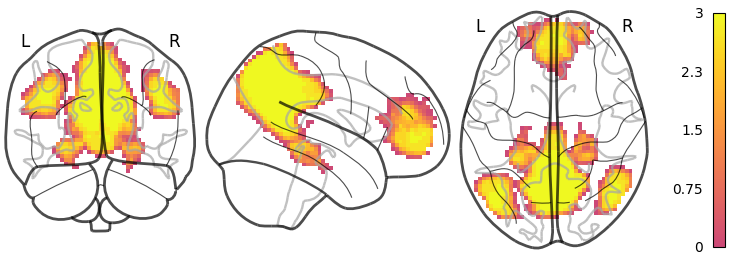
\includegraphics[width=0.33\linewidth,height=0.3\textheight]{../report/fig/DMN_thresholded_for_clusterFWE005} }\subfloat[Reward network seeded from Nucleus Accumbens\label{fig:figNetworks-2}]{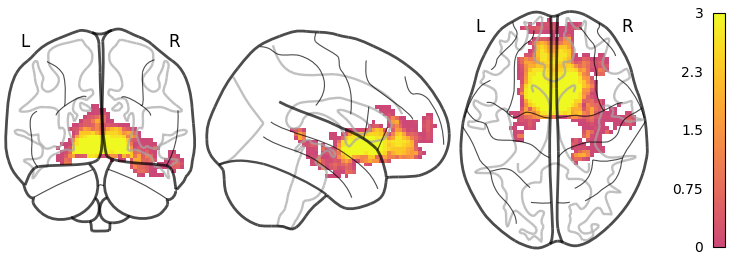
\includegraphics[width=0.33\linewidth,height=0.3\textheight]{../report/fig/Rew_thresholded_for_clusterFWE005} }\subfloat[tSNR differences between regions\label{fig:figNetworks-3}]{\includegraphics[width=0.33\linewidth,height=0.3\textheight]{../report/tsnr} }

}

\caption{Resting state networks based on AROMA+CC+GSR input data, one-sample t-tests adjusting for age and sex over all timepoints and participants with bootstrapped clusterwise inference (p FWE<0.05)}\label{fig:figNetworks}
\end{figure}

Figure \ref{fig:figNetworks} shows the DMN and reward network average maps which we used for extracting aggregated FC values. Both networks included the typically described brain regions (i.e.~medial prefrontal cortex, parietal lobules and posterior hippocampus for the DMN, and anterior cingulate, right amygdala and ventromedial-prefrontal cortex for the reward network).
Yet, the reward network was less pronounced (overall lower T-values) and symmetric (no significant connectivity with left amygdala), which might be due to lower SNR in the seeded brain region (see Figure \ref{fig:figNetworks}).

\hypertarget{interaction-effect-of-intervention-and-time-preregistered-analysis}{%
\subsection{Interaction effect of intervention and time (preregistered analysis)}\label{interaction-effect-of-intervention-and-time-preregistered-analysis}}

\hypertarget{dmnreward-network-with-whole-brain-mask-preregistered-analysis}{%
\subsubsection{DMN/reward network with whole brain mask (preregistered analysis)}\label{dmnreward-network-with-whole-brain-mask-preregistered-analysis}}

\hypertarget{model-1a-with-adjustment-for-age-sex}{%
\paragraph{Model 1a (with adjustment for age, sex)}\label{model-1a-with-adjustment-for-age-sex}}

Against our initial hypothesis, there was no interaction effect of group and time point for FC for neither the PCC nor the NAcc seeds. There also was no significant main effect for any of the covariates of interest (time, group) in clusterwise inference with FWE correction.

\hypertarget{model-1b-with-adjustment-for-age-and-sex-meanfd}{%
\paragraph{Model 1b (with adjustment for age and sex, meanFD)}\label{model-1b-with-adjustment-for-age-and-sex-meanfd}}

Similarly, there were no significant clusters when including mFD. Results did not differ between AROMA+CC and AROMA+CC+GSR preprocessing pipelines.

Unthresholded maps for the t-tests of the DMN and reward network (which were used for data aggregation) as well as contrasts of group, time and group-by-time interaction are on \href{insert\%20link\%20here}{NeuroVault}.

\hypertarget{interaction-effect-group-by-time-on-aggregated-fc-preregistered-analysis}{%
\subsection{Interaction effect group by time on aggregated FC (preregistered analysis)}\label{interaction-effect-group-by-time-on-aggregated-fc-preregistered-analysis}}

There was no significant time by group interaction for aggregated DMN and reward network FC (see Figures \ref{fig:figaggDMN} and \ref{fig:figaggRew} and supplements for a detailed summary of the models)

\begin{figure}
\includegraphics[width=0.75\linewidth]{draft_rsfmri_files/figure-latex/figaggDMN-1} \caption{DMN connectivity per group over time}\label{fig:figaggDMN}
\end{figure}

\begin{figure}
\includegraphics[width=0.75\linewidth]{draft_rsfmri_files/figure-latex/figaggRew-1} \caption{Reward network connectivity per group over time}\label{fig:figaggRew}
\end{figure}

\begin{verbatim}
##    mean_DMN_conn mean_Rew_conn subj.ID_tp subj.ID  tp condition
## 2       0.063282      0.072570 ADI003_fu2  ADI003 fu2        IG
## 34      0.073654      0.038568  ADI041_fu  ADI041  fu        KG
\end{verbatim}

\begin{verbatim}
##   X subj.ID  tp Age_BL  Sex  BMI condition longtemplate.run long.runs
## 6 6  ADI003 fu2     53 male 40.9        IG                1         1
##   T1.comments DWI.comments rs.comments Preprocessed rs.QA.residuals rs.QA.GM
## 6                                                 1               1        0
##   rs.Qa.carpetplots.comment    Subject Exclude Final_Score Excessive_motion
## 6                        NA ADI003_fu2      NA           3                0
##   Temp_pole_missing_rh Temp_pole_miss_lh Dura_rh Dura_lh
## 6                    1                 0       1       1
##                                Check_comments Correction.done
## 6 dura: lh: sl 45-50; rh: 146:149, rh TL: 136               1
##                            Correction_comments Missing_Anterior_rh
## 6 corrected pial, wm rh temporal lobe manually                   0
##   Missing_Anterior_lh Missing_Superior_medial_rh Missing_Superior_Medial_lh
## 6                   0                          0                          0
##   Missing_Posterior_rh Missing_Posterior_lh long.timepoints_check    meanFD
## 6                    0                    0                    ok 0.1793491
##       maxFD original_tp
## 6 0.7365457         fu2
\end{verbatim}

\begin{verbatim}
##     X subj.ID tp Age_BL    Sex  BMI condition longtemplate.run long.runs
## 56 56  ADI041 fu     68 female 45.5        KG                1         1
##    T1.comments DWI.comments rs.comments Preprocessed rs.QA.residuals rs.QA.GM
## 56                                                 1               0        0
##    rs.Qa.carpetplots.comment   Subject Exclude Final_Score Excessive_motion
## 56                        NA ADI041_fu      NA           3                1
##    Temp_pole_missing_rh Temp_pole_miss_lh Dura_rh Dura_lh Check_comments
## 56                    0                 0       0       0               
##    Correction.done Correction_comments Missing_Anterior_rh Missing_Anterior_lh
## 56               1                                       0                   0
##    Missing_Superior_medial_rh Missing_Superior_Medial_lh Missing_Posterior_rh
## 56                          0                          0                    0
##    Missing_Posterior_lh long.timepoints_check    meanFD    maxFD original_tp
## 56                    0                    ok 0.5251626 1.153295          fu
\end{verbatim}

\begin{verbatim}
##    mean_Rew_conn subj.ID_tp subj.ID  tp condition
## 64      0.363538  ADI069_bl  ADI069  bl        IG
## 90      0.362268 ADI111_fu2  ADI111 fu2        KG
\end{verbatim}

\includegraphics{draft_rsfmri_files/figure-latex/identify outliers in these plots-1.pdf}

\begin{verbatim}
##     X subj.ID tp Age_BL    Sex  BMI condition longtemplate.run long.runs
## 93 94  ADI069 bl     52 female 45.6        IG                1         1
##    T1.comments DWI.comments rs.comments Preprocessed rs.QA.residuals rs.QA.GM
## 93                                                 1               1        1
##    rs.Qa.carpetplots.comment   Subject Exclude Final_Score Excessive_motion
## 93                        NA ADI069_bl      NA           2                0
##    Temp_pole_missing_rh Temp_pole_miss_lh Dura_rh Dura_lh
## 93                    0                 0       1       1
##                       Check_comments Correction.done Correction_comments
## 93 around slice 130 brain is missing               1                    
##    Missing_Anterior_rh Missing_Anterior_lh Missing_Superior_medial_rh
## 93                   0                   0                          0
##    Missing_Superior_Medial_lh Missing_Posterior_rh Missing_Posterior_lh
## 93                          0                    0                    0
##                                                                                                     long.timepoints_check
## 93 could be further corrected but no large parts of skull in brainmask, especially fu2 includes more skull but also other
##       meanFD    maxFD original_tp
## 93 0.3246258 1.250849          bl
\end{verbatim}

\begin{verbatim}
##       X subj.ID  tp Age_BL    Sex   BMI condition longtemplate.run long.runs
## 134 135  ADI111 fu2     45 female 38.86        KG                1         1
##     T1.comments DWI.comments rs.comments Preprocessed rs.QA.residuals rs.QA.GM
## 134                                                 1               1        1
##     rs.Qa.carpetplots.comment    Subject Exclude Final_Score Excessive_motion
## 134                        NA ADI111_fu2      NA           1                0
##     Temp_pole_missing_rh Temp_pole_miss_lh Dura_rh Dura_lh Check_comments
## 134                    0                 0       0       0               
##     Correction.done Correction_comments Missing_Anterior_rh Missing_Anterior_lh
## 134              NA                                       0                   0
##     Missing_Superior_medial_rh Missing_Superior_Medial_lh Missing_Posterior_rh
## 134                          0                          0                    0
##     Missing_Posterior_lh long.timepoints_check    meanFD     maxFD original_tp
## 134                    0                       0.2217564 0.6373868         fu2
\end{verbatim}

There was no significant time by group interaction effect for aggregated DMN and reward network FC (see Figures \ref{fig:figaggDMN} and \ref{fig:figaggRew} and supplements for a detailed summary of the models).

\includegraphics{draft_rsfmri_files/figure-latex/qa check DMN model age,sex-1.pdf} \includegraphics{draft_rsfmri_files/figure-latex/qa check DMN model age,sex-2.pdf}

\begin{verbatim}
## [1] "please carefully evaluate whether the result makes sense, and if not, please contact me"
\end{verbatim}

\begin{verbatim}
## 
## none 
##   46
\end{verbatim}

\begin{verbatim}
##                                          what          orig           min
## (Intercept)                       (Intercept)  0.3011366890  0.2882606175
## tpfu                                     tpfu -0.0042961373 -0.0075864874
## group_factorKG                 group_factorKG -0.0301407218 -0.0377386050
## Age_BL                                 Age_BL -0.0003086131 -0.0006174032
## Sex                                       Sex -0.0072143466 -0.0103655403
## subj.ID@(Intercept)@NA subj.ID@(Intercept)@NA  0.0102987605  0.0000000000
## Residual                             Residual  0.0589888164  0.0440983541
##                                  max
## (Intercept)             3.133646e-01
## tpfu                    4.638475e-03
## group_factorKG         -2.132058e-02
## Age_BL                 -6.008462e-05
## Sex                    -4.407144e-03
## subj.ID@(Intercept)@NA  2.819585e-02
## Residual                5.853199e-02
\end{verbatim}

\includegraphics{draft_rsfmri_files/figure-latex/qa check DMN model age,sex, mFD-1.pdf} \includegraphics{draft_rsfmri_files/figure-latex/qa check DMN model age,sex, mFD-2.pdf}

\begin{verbatim}
## [1] "please carefully evaluate whether the result makes sense, and if not, please contact me"
\end{verbatim}

\begin{verbatim}
## 
## none 
##   46
\end{verbatim}

\begin{verbatim}
##                                          what          orig           min
## (Intercept)                       (Intercept)  0.2882310534  0.2712944647
## tpfu                                     tpfu -0.0054314895 -0.0100474095
## group_factorKG                 group_factorKG -0.0288732597 -0.0371734358
## Age_BL                                 Age_BL -0.0001981959 -0.0004808581
## Sex                                       Sex -0.0062543208 -0.0094973527
## logmFD                                 logmFD -0.0133761940 -0.0311612579
## subj.ID@(Intercept)@NA subj.ID@(Intercept)@NA  0.0144570585  0.0000000000
## Residual                             Residual  0.0585590452  0.0437893877
##                                  max
## (Intercept)             3.043966e-01
## tpfu                    3.891318e-03
## group_factorKG         -1.942998e-02
## Age_BL                  3.457184e-05
## Sex                    -3.092665e-03
## logmFD                  1.596906e-03
## subj.ID@(Intercept)@NA  2.873301e-02
## Residual                5.837731e-02
\end{verbatim}

\includegraphics{draft_rsfmri_files/figure-latex/qa check Rew model age,sex-1.pdf} \includegraphics{draft_rsfmri_files/figure-latex/qa check Rew model age,sex-2.pdf}

\begin{verbatim}
## [1] "please carefully evaluate whether the result makes sense, and if not, please contact me"
\end{verbatim}

\begin{verbatim}
## 
## none 
##   46
\end{verbatim}

\begin{verbatim}
##                                          what          orig           min
## (Intercept)                       (Intercept)  0.1233716391  0.1027031052
## tpfu                                     tpfu -0.0035148229 -0.0070886207
## group_factorKG                 group_factorKG -0.0107355182 -0.0230637231
## Age_BL                                 Age_BL  0.0004245927  0.0001949297
## Sex                                       Sex -0.0058271841 -0.0107320399
## subj.ID@(Intercept)@NA subj.ID@(Intercept)@NA  0.0368043138  0.0285664602
## Residual                             Residual  0.0541471334  0.0428115665
##                                  max
## (Intercept)             0.1359575360
## tpfu                    0.0040817069
## group_factorKG         -0.0048054540
## Age_BL                  0.0008687551
## Sex                    -0.0021879107
## subj.ID@(Intercept)@NA  0.0387259006
## Residual                0.0541921574
\end{verbatim}

\includegraphics{draft_rsfmri_files/figure-latex/qa check Rew model age, sex, mFD-1.pdf} \includegraphics{draft_rsfmri_files/figure-latex/qa check Rew model age, sex, mFD-2.pdf}

\begin{verbatim}
## [1] "please carefully evaluate whether the result makes sense, and if not, please contact me"
\end{verbatim}

\begin{verbatim}
## 
## none 
##   46
\end{verbatim}

\begin{verbatim}
##                                          what          orig           min
## (Intercept)                       (Intercept)  0.0662061153  0.0446574064
## tpfu                                     tpfu -0.0084837422 -0.0108942561
## group_factorKG                 group_factorKG -0.0051835290 -0.0180592427
## Age_BL                                 Age_BL  0.0009275477  0.0005888916
## Sex                                       Sex -0.0014919066 -0.0066504423
## logmFD                                 logmFD -0.0586481745 -0.0700504675
## subj.ID@(Intercept)@NA subj.ID@(Intercept)@NA  0.0387074827  0.0306199614
## Residual                             Residual  0.0522837751  0.0415234010
##                                  max
## (Intercept)             0.0927661360
## tpfu                   -0.0007931101
## group_factorKG          0.0011426393
## Age_BL                  0.0012776894
## Sex                     0.0021175666
## logmFD                 -0.0414794258
## subj.ID@(Intercept)@NA  0.0384413597
## Residual                0.0522319920
\end{verbatim}

\hypertarget{exploratory-analyses}{%
\subsection{Exploratory Analyses}\label{exploratory-analyses}}

\hypertarget{effect-of-mean-and-change-in-bmi}{%
\subsubsection{Effect of mean and change in BMI}\label{effect-of-mean-and-change-in-bmi}}

\hypertarget{whole-brain-analysis}{%
\paragraph{Whole brain analysis}\label{whole-brain-analysis}}

\hypertarget{bmi-only-model}{%
\subparagraph{BMI-only model}\label{bmi-only-model}}

Next, we tested for significant effects of the average BMI and the individual change in BMI longitudinally across the three time points.
Using the images preprocessed with AROMA+CC, we found a significant negative association of average BMI and DMN connectivity in the lingual gyrus, mid orbital gyrus and temporal gyrus, which remained stable after including mFD as nuisance covariate (FWE cluster p\textless0.05). When using GSR preprocessed data, none of the clusters was significantly associated with average BMI (Table \ref{tab:tableBMImodel}.

\begin{figure}
\subfloat[adjusted for age and sex\label{fig:BMIagesexPCCccavgBMIdeact-1}]{\includegraphics[width=0.5\linewidth]{../report/fig/BMIagesex_PCCcc_avgBMI_deact} }\subfloat[adjusted for age, sex and mFD\label{fig:BMIagesexPCCccavgBMIdeact-2}]{\includegraphics[width=0.5\linewidth]{../report/fig/BMIagesexfd_PCCcc_avgBMI_deact} }\caption{Negative association of average BMI and FC with PCC/precuneus in AROMA+CC preprocessed data}\label{fig:BMIagesexPCCccavgBMIdeact}
\end{figure}

NAcc connectivity was not significantly related to neither mean nor change in BMI, for either of the preprocessing schemes.
Results with significant cluster co-activation are depicted in Table \ref{tab:tableBMImodel}.

\hypertarget{bmi-and-fd-model}{%
\subparagraph{BMI and FD model}\label{bmi-and-fd-model}}

To disentangle effects of change in BMI and mFD in this dataset, we split mFD into average mFD and change in mFD. Age and sex were kept as nuisance covariates.
Average BMI remained significantly negatively associated with the three clusters above when splitting FD into its components. Results are detailed in Table \ref{tab:tableBMIFDmodel}.
Test statistics only differed slightly from the effect found when using mFD as nuisance covariate.
As before, the effect did not survive when using GSR-corrected data.

For the reward network, we found a significant negative association of change in BMI with FC between NAcc and a cluster in the posterior-medial frontal region, i.e.~supplementary motor area (see Table \ref{tab:tableBMIFDmodel}). Voxel activation at local maximum within this cluster was significant at peak level after FWE-correction (p=\(0.028\)), also when evaluating the GSR corrected data (p=\(0.038\)).

\begin{figure}
\subfloat[in AROMA+CC\label{fig:BMIFDagesexNACCcgnBMIdeact-1}]{\includegraphics[width=0.5\linewidth]{../report/fig/BMIFDagesex_NACCcc_cngBMI_deact} }\subfloat[in AROMA+CC+GSR data\label{fig:BMIFDagesexNACCcgnBMIdeact-2}]{\includegraphics[width=0.5\linewidth]{../report/fig/BMIFDagesex_NACCgsr_cngBMI_deact} }\caption{Significant cluster with a negative Effect of change BMI on NAcc to posterior-medial frontal region, adjusted for age, sex, mean BMI and mFD}\label{fig:BMIFDagesexNACCcgnBMIdeact}
\end{figure}

Moreover, FC between the NAcc and one cluster in a more posterior region, i.e.~motor cortex, was significantly positively related to average mFD. This result remained similar when using GSR corrected data.

\begin{figure}
\subfloat[in AROMA+CC\label{fig:BMIFDagesexNACCavgFDact-1}]{\includegraphics[width=0.5\linewidth]{../report/fig/BMIFDagesex_NACCcc_avgFD_act} }\subfloat[in AROMA+CC+GSR data\label{fig:BMIFDagesexNACCavgFDact-2}]{\includegraphics[width=0.5\linewidth]{../report/fig/BMIFDagesex_NACCgsr_avgFD_act} }\caption{Significant cluster with a positive Effect of average mFD on connectivity between NAcc and motor cortex, adjusted for age, sex, mean BMI, change in BMI and change in mFD}\label{fig:BMIFDagesexNACCavgFDact}
\end{figure}

\hypertarget{aggregated-fc-analysis-1}{%
\paragraph{Aggregated FC analysis}\label{aggregated-fc-analysis-1}}

Corresponding to the whole brain results, there was a negative association of mean BMI and aggregated DMN connectivity (p = 0.012), regardless of whether we adjusted for mFD.

The association also remained significant when we split mFD into average and change in mFD (p = NA, 0.0122) and there was no significant association of mean or change in mFD with DMN FC.

\hypertarget{reward-network-mean-and-within-variability-in-bmi-and-logmfd}{%
\paragraph{Reward network, mean and within variability in BMI and logmFD}\label{reward-network-mean-and-within-variability-in-bmi-and-logmfd}}

As expected from the whole-brain findings, there was no association of mean BMI or within-subject BMI change and reward network connectivity in models adjusting for age, sex and mFD.

\hypertarget{effect-of-fd-exploratory-analysis}{%
\subsubsection{Effect of FD (exploratory analysis)}\label{effect-of-fd-exploratory-analysis}}

\hypertarget{whole-brain-analysis-1}{%
\paragraph{Whole-brain analysis}\label{whole-brain-analysis-1}}

To investigate the unique contributions of the average value of and the longitudinal change in mFD, we constructed two additional models.
First, BMI measures are excluded from the design matrix. Covariance of the mFD and outcome measures is investigated by splitting mFD into average mFD and longitudinal mFD change and by inspecting associations with each predictor. Age and sex were nuisance covariates.

As shown in Table \ref{tab:tableFDmodel}, there was a significant association between mFD and co-activation of NAcc with one cluster located in proximity to the central sulcus and motor areas . Cluster co-activation appeared irrespective of the preprocessing procedure, differing mainly in cluster size.
We did not find a any clusters for functional connectivity with the PCC.

\begin{figure}
\subfloat[in AROMA+CC\label{fig:FDagesexNACCccavgFDact-1}]{\includegraphics[width=0.5\linewidth]{../report/fig/FDagesex_NACCcc_avgFD_act} }\subfloat[in AROMA+CC+GSR data\label{fig:FDagesexNACCccavgFDact-2}]{\includegraphics[width=0.5\linewidth]{../report/fig/FDagesex_NACCgsr_avgFD_act} }\caption{Positive association of mean mFD and FC of NAcc with cluster, adjusted for age, sex, mean BMI, change BMI and change mFD}\label{fig:FDagesexNACCccavgFDact}
\end{figure}

\hypertarget{effect-of-bmi-and-fd-exploratory-analysis}{%
\subsection{Effect of BMI and FD (exploratory analysis)}\label{effect-of-bmi-and-fd-exploratory-analysis}}

Average BMI and change in BMI remain covariates of interest. While initially used as nuisance covariate, here, mFD is split into average mFD and change in mFD and used as. Age and sex remain nuisance covariates.

There is a significant effect of change in BMI on functional connectivity between NAcc and one cluster in the posterior-medial frontal region.
Voxel activation at local maximum within this cluster was significant at peak level after FWE-correction. Furthermore, the functional connectivity between the NAcc and one cluster was significantly related to average mFD.
When running the model with images corrected with GSR, the associations between connectivity and change in BMI did not survive statistical thresholds.
On the other hand, the relationship with average mFD was confirmed by analyses after GSR but cluster size shrank.

\begin{landscape}\begin{table}

\caption{\label{tab:tableBMImodel}Changes in functional connectivity in whole brain analysis for BMI model}
\centering
\resizebox{\linewidth}{!}{
\begin{tabular}[t]{llrrrrrrrll}
\toprule
\multicolumn{1}{c}{ } & \multicolumn{1}{c}{ } & \multicolumn{3}{c}{clusterwise¹} & \multicolumn{6}{c}{voxelwise  at local maximum} \\
\cmidrule(l{3pt}r{3pt}){3-5} \cmidrule(l{3pt}r{3pt}){6-11}
\multicolumn{6}{c}{ } & \multicolumn{3}{c}{MNI coordinates} \\
\cmidrule(l{3pt}r{3pt}){7-9}
Seed & Covariates & FWE-corr. P & cluster size & Z score & FWE-corr. P & X & Y & Z & Hem & Anatomical region²\\
\midrule
\addlinespace[0.3em]
\multicolumn{11}{l}{\textbf{average BMI (decrease)}}\\
\hspace{1em}PCC (cc) & age, sex & 0.002 & 204 & 1.756 & 0.010 & -6 & -30 & -3 &  & -\\
\hspace{1em}NA & NA & NA & NA & NA & 0.061 & -3 & -45 & 6 &  & -\\
\hspace{1em}NA & NA & NA & NA & NA & 0.065 & 12 & -39 & 0 & R & Lingual Gyrus\\
\hspace{1em}NA & NA & 0.026 & 74 & 1.610 & 0.089 & -51 & -9 & -12 & R & Mid Orbital Gyrus\\
\hspace{1em}NA & NA & NA & NA & NA & 0.369 & -54 & 0 & -21 & L & Mid Orbital Gyrus\\
\hspace{1em}NA & NA & NA & NA & NA & 0.377 & -57 & -3 & -12 & L & Mid Orbital Gyrus\\
\hspace{1em}NA & NA & 0.026 & 75 & 1.612 & 0.226 & 9 & 54 & -6 & L & Superior Temporal Gyrus\\
\hspace{1em}NA & NA & NA & NA & NA & 0.268 & -3 & 57 & -12 & L & Middle Temporal Gyrus\\
\hspace{1em}NA & NA & 0.036 & 63 & 1.580 & 0.303 & 60 & -12 & -6 & R & Superior Temporal Gyrus\\
\hspace{1em}NA & NA & NA & NA & NA & 0.643 & 66 & -21 & -9 & R & Middle Temporal Gyrus\\
\addlinespace[0.3em]
\multicolumn{11}{l}{\textbf{average BMI (decrease)}}\\
\hspace{1em}PCC (cc) & age, sex, log mFD & 0.001 & 233 & 1.765 & 0.011 & -6 & -30 & -3 &  & -\\
\hspace{1em}NA & NA & NA & NA & NA & 0.062 & -3 & -45 & 6 &  & -\\
\hspace{1em}NA & NA & NA & NA & NA & 0.063 & 12 & -39 & 0 & R & Lingual Gyrus\\
\hspace{1em}NA & NA & 0.039 & 73 & 1.603 & 0.074 & -51 & -9 & -12 & L & Mid Orbital Gyrus\\
\hspace{1em}NA & NA & NA & NA & NA & 0.337 & -54 & -3 & -21 & R & Mid Orbital Gyrus\\
\hspace{1em}NA & NA & 0.036 & 80 & 1.619 & 0.206 & 0 & 60 & -12 & L & Superior Temporal Gyrus\\
\hspace{1em}NA & NA & NA & NA & NA & 0.241 & 9 & 54 & -6 & L & Middle Temporal Gyrus\\
\hspace{1em}NA & NA & NA & NA & NA & 0.376 & -6 & 51 & -9 & R & Superior Temporal Gyrus\\
\hspace{1em}NA & NA & 0.049 & 57 & 1.556 & 0.279 & 60 & -12 & -6 & R & Superior Temporal Gyrus\\
\hspace{1em}NA & NA & NA & NA & NA & 0.660 & 66 & -21 & -9 & R & Middle Temporal Gyrus\\
\bottomrule
\multicolumn{11}{l}{\textsuperscript{} Hem, hemisphere; L, left; R, right; FWE-corr., family-wise error corrected; MNI (Montreal Neurological Institute) coordinates of}\\
\multicolumn{11}{l}{primary peak location: X sagittal; Y, coronal; Z, axial; cc, preprocessing with AROMA-ICA + CompCor; gsr, preprocessing with}\\
\multicolumn{11}{l}{AROMA-ICA + CompCor + GSR.}\\
\multicolumn{11}{l}{\textsuperscript{1} To identify significant clusters, we applied a cluster size threshold with p < 0.001 determined by Wild Bootstrap of 1000}\\
\multicolumn{11}{l}{samples.}\\
\multicolumn{11}{l}{\textsuperscript{2} Connectivity with maximum three voxels that mark local maxima within the respective custer; more detailed description of}\\
\multicolumn{11}{l}{anatomical regions that are assigned to overall clusters and and corresponding probability in Supplementary.}\\
\end{tabular}}
\end{table}
\end{landscape}

\begin{landscape}\begin{table}

\caption{\label{tab:tableFDmodel}Changes in functional connectivity in whole brain analysis for FD model}
\centering
\resizebox{\linewidth}{!}{
\begin{tabular}[t]{llrrrrrrrll}
\toprule
\multicolumn{1}{c}{ } & \multicolumn{1}{c}{ } & \multicolumn{3}{c}{clusterwise¹} & \multicolumn{6}{c}{voxelwise  at local maximum} \\
\cmidrule(l{3pt}r{3pt}){3-5} \cmidrule(l{3pt}r{3pt}){6-11}
\multicolumn{6}{c}{ } & \multicolumn{3}{c}{MNI coordinates} \\
\cmidrule(l{3pt}r{3pt}){7-9}
Seed & Covariates & FWE-corr. P & cluster size & Z score & FWE-corr. P & X & Y & Z & Hem & Anatomical region²\\
\midrule
\addlinespace[0.3em]
\multicolumn{11}{l}{\textbf{average log mean FD (increase)}}\\
\hspace{1em}NAcc (cc) & age, sex & 0.008 & 151 & 1.606 & 0.052 & 9 & -15 & 60 & R & Posterior-Medial Frontal\\
\hspace{1em}NA & NA & NA & NA & NA & 0.265 & 12 & -27 & 63 & R & Paracentral Lobule\\
\hspace{1em}NA & NA & NA & NA & NA & 0.360 & -6 & -24 & 51 & L & Paracentral Lobule\\
\addlinespace[0.3em]
\multicolumn{11}{l}{\textbf{average log mean FD (increase)}}\\
\hspace{1em}NAcc (gsr) & age, sex & 0.017 & 57 & 1.812 & 0.131 & 9 & -15 & 60 & R & Posterior-Medial Frontal\\
\hspace{1em}NA & NA & NA & NA & NA & 0.561 & 9 & -6 & 72 & R & Posterior-Medial Frontal\\
\bottomrule
\multicolumn{11}{l}{\textsuperscript{} Hem, hemisphere; L, left; R, right; FWE-corr., family-wise error corrected; MNI (Montreal Neurological Institute) coordinates of}\\
\multicolumn{11}{l}{primary peak location: X sagittal; Y, coronal; Z, axial; cc, preprocessing with AROMA-ICA + CompCor; gsr, preprocessing with}\\
\multicolumn{11}{l}{AROMA-ICA + CompCor + GSR.}\\
\multicolumn{11}{l}{\textsuperscript{1} To identify significant clusters, we applied a cluster size threshold with p < 0.001 determined by Wild Bootstrap of 1000}\\
\multicolumn{11}{l}{samples.}\\
\multicolumn{11}{l}{\textsuperscript{2} Connectivity with maximum three voxels that mark local maxima within the respective custer; more detailed description of}\\
\multicolumn{11}{l}{anatomical regions that are assigned to overall clusters and and corresponding probability in Supplementary.}\\
\end{tabular}}
\end{table}
\end{landscape}

\begin{landscape}\begin{table}

\caption{\label{tab:tableBMIFDmodel}Changes in functional connectivity in whole brain analysis for BMI-FD model}
\centering
\resizebox{\linewidth}{!}{
\begin{tabular}[t]{llrrrrrrrll}
\toprule
\multicolumn{1}{c}{ } & \multicolumn{1}{c}{ } & \multicolumn{3}{c}{clusterwise¹} & \multicolumn{6}{c}{voxelwise  at local maximum} \\
\cmidrule(l{3pt}r{3pt}){3-5} \cmidrule(l{3pt}r{3pt}){6-11}
\multicolumn{6}{c}{ } & \multicolumn{3}{c}{MNI coordinates} \\
\cmidrule(l{3pt}r{3pt}){7-9}
Seed & Covariates & FWE-corr. P & cluster size & Z score & FWE-corr. P & X & Y & Z & Hem & Anatomical region²\\
\midrule
\addlinespace[0.3em]
\multicolumn{11}{l}{\textbf{change in BMI (decrease)}}\\
\hspace{1em}NAcc (cc) & age, sex & 0.028 & 108 & 1.648 & 0.038 & 0 & 3 & 66 & L & Posterior-Medial Frontal\\
\hspace{1em}NA & NA & NA & NA & NA & 0.649 & -3 & 12 & 66 & R & Posterior-Medial Frontal\\
\addlinespace[0.3em]
\multicolumn{11}{l}{\textbf{average log mean FD (increase)}}\\
\hspace{1em}NAcc (cc) & age, sex & 0.003 & 177 & 1.998 & 0.010 & 9 & -15 & 60 & R & Posterior-Medial Frontal\\
\hspace{1em}NA & NA & NA & NA & NA & 0.076 & 12 & -27 & 63 & R & Paracentral Lobule\\
\hspace{1em}NA & NA & NA & NA & NA & 0.376 & -6 & -24 & 51 & L & Paracentral Lobule\\
\addlinespace[0.3em]
\multicolumn{11}{l}{\textbf{change in BMI (decrease)}}\\
\hspace{1em}NAcc (gsr) & age, sex & 0.038 & 92 & 1.665 & 0.134 & 6 & 9 & 63 & R & Posterior-Medial Frontal\\
\hspace{1em}NA & NA & NA & NA & NA & 0.468 & 0 & 3 & 66 & L & Posterior-Medial Frontal\\
\addlinespace[0.3em]
\multicolumn{11}{l}{\textbf{average log mean FD (increase)}}\\
\hspace{1em}NAcc (gsr) & age, sex & 0.007 & 71 & 1.807 & 0.091 & 9 & -15 & 60 & R & Posterior-Medial Frontal\\
\hspace{1em}NA & NA & NA & NA & NA & 0.356 & 3 & -6 & 51 & R & Posterior-Medial Frontal\\
\hspace{1em}NA & NA & NA & NA & NA & 0.638 & 9 & -6 & 72 & R & Posterior-Medial Frontal\\
\addlinespace[0.3em]
\multicolumn{11}{l}{\textbf{average BMI (decrease)}}\\
\hspace{1em}PCC (cc) & age, sex & 0.001 & 246 & 1.794 & 0.011 & -6 & -30 & -3 &  & -\\
\hspace{1em}NA & NA & NA & NA & NA & 0.047 & -3 & -45 & 6 &  & -\\
\hspace{1em}NA & NA & NA & NA & NA & 0.051 & 12 & -39 & 0 & R & Lingual Gyrus\\
\hspace{1em}NA & NA & 0.032 & 72 & 1.617 & 0.063 & -51 & -9 & -12 & R & Mid Orbital Gyrus\\
\hspace{1em}NA & NA & NA & NA & NA & 0.340 & -54 & -3 & -21 & L & Mid Orbital Gyrus\\
\hspace{1em}NA & NA & 0.021 & 90 & 1.657 & 0.165 & 9 & 54 & -6 & L & Superior Temporal Gyrus\\
\hspace{1em}NA & NA & NA & NA & NA & 0.187 & 0 & 60 & -12 & L & Middle Temporal Gyrus\\
\hspace{1em}NA & NA & NA & NA & NA & 0.294 & -6 & 51 & -9 &  & NA\\
\bottomrule
\multicolumn{11}{l}{\textsuperscript{} Hem, hemisphere; L, left; R, right; FWE-corr., family-wise error corrected; MNI (Montreal Neurological Institute) coordinates of}\\
\multicolumn{11}{l}{primary peak location: X sagittal; Y, coronal; Z, axial; cc, preprocessing with AROMA-ICA + CompCor; gsr, preprocessing with}\\
\multicolumn{11}{l}{AROMA-ICA + CompCor + GSR.}\\
\multicolumn{11}{l}{\textsuperscript{1} To identify significant clusters, we applied a cluster size threshold with p < 0.001 determined by Wild Bootstrap of 1000}\\
\multicolumn{11}{l}{samples.}\\
\multicolumn{11}{l}{\textsuperscript{2} Connectivity with maximum three voxels that mark local maxima within the respective custer; more detailed description of}\\
\multicolumn{11}{l}{anatomical regions that are assigned to overall clusters and and corresponding probability in Supplementary.}\\
\end{tabular}}
\end{table}
\end{landscape}

The effect of average BMI on connectivity between the PCC and other regions reported previously is confirmed. There is a significant association between average BMI and the connectivity between PCC and three other clusters. Results are detailed in Table \ref{tab:tableBMIFDmodel}.
Test statistics of these clusters differ only slightly from the effect found for average BMI when using mFD as nuisance covariate.
As before, the effect did not survive when thresholding if the images had been GSR corrected.
\textbackslash begin\{figure\}
\subfloat[in AROMA+CC(\#fig:BMIFDagesex_NACC_avgFD_act-1)]{\includegraphics[width=0.5\linewidth]{../report/fig/BMIFDagesex_NACCcc_avgFD_act} }\subfloat[in AROMA+CC+GSR data(\#fig:BMIFDagesex_NACC_avgFD_act-2)]{\includegraphics[width=0.5\linewidth]{../report/fig/BMIFDagesex_NACCgsr_avgFD_act} }

\caption{Positive association of mean mFD and FC of NAcc with cluster, adjusted for age, sex, average BMI, change BMI and change mFD}

(\#fig:BMIFDagesex\_NACC\_avgFD\_act)
\textbackslash end\{figure\}

\textbackslash begin\{figure\}
\subfloat[in AROMA+CC(\#fig:BMIFDagesex_NACC_cgnBMI_deact-1)]{\includegraphics[width=0.5\linewidth]{../report/fig/BMIFDagesex_NACCcc_cngBMI_deact} }\subfloat[in AROMA+CC+GSR data(\#fig:BMIFDagesex_NACC_cgnBMI_deact-2)]{\includegraphics[width=0.5\linewidth]{../report/fig/BMIFDagesex_NACCgsr_cngBMI_deact} }

\caption{Positive association of change in BMI and FC of NAcc with cluster, adjusted for age, sex, average BMI, average mFD and change mFD}

(\#fig:BMIFDagesex\_NACC\_cgnBMI\_deact)
\textbackslash end\{figure\}

\includegraphics[width=0.75\linewidth]{../report/fig/BMIFDagesex_PCCcc_avgBMI_deact}

\hypertarget{effect-on-hypothalamic-connectivity-exploratory-analysis}{%
\subsection{Effect on hypothalamic connectivity (exploratory analysis)}\label{effect-on-hypothalamic-connectivity-exploratory-analysis}}

\ldots{}

Unthresholded maps for the t-tests as well as contrasts of average BMI and change BMI of the main model, and post-hoc contrasts for average FD and change FD will be are published on NeuroVault.

\hypertarget{discussion}{%
\section{Discussion}\label{discussion}}

\hypertarget{summary}{%
\paragraph{Summary}\label{summary}}

Utilizing resting-state functional MRI on morbidly obese individuals that either underwent or awaited bariatric surgery over the course of one year.
Building on the evidence for post-surgery changes in functional activity, this study explored the longitudinal relationship between surgery-induced weight loss and functional integrity in target networks indicated by resting-state functional connectivity. Over the course of one year we collected neuroimaging and anthropometric data from 33 morbidly obese patients undergoing bariatric surgery and compared them to the longitudinal data of 15 patients on the waiting list.
Looking at time-by-group interactions, we primarily investigated whether changes in functional connectivity over time vary depending whether participants have received surgery or not, while controlling for individual variance in resting-state connectivity over time and at baseline. Beyond that, main effects of the intervention and of the time were examined.
The second model further investigates if changes in connectivity are a function of an average BMI (controlled for individual variance in BMI) and the longitudinal change in BMI.
To get a better understanding of our results, we conducted multiverse exploratory analyses representing different choices regarding preprocessing pipelines, inclusion of covariates and subsets of the data relevant for interpretation.

\hypertarget{support-of-original-hypotheses}{%
\paragraph{Support of original hypotheses}\label{support-of-original-hypotheses}}

To summarize, while our primary hypothesis on group time interactions could not be confirmed, there was a significant relationship between functional activation
and the continuous BMI measures for some but not all analyses.

\begin{itemize}
\tightlist
\item
  DMN: average BMI but only with lenient AROMA-CC but then for both covariate structures age/sex/mFD and age/sex; effect stable when separating avg mFD and cgn FD into two regressors
\item
  Reward: effect of change BMI only when separating mFD, bit high peak activation
  The individuals BMI averaged across measures taken throughout the one-year period negatively correlated with functional connectivity between PCC and {[}regions from clusters{]}. Results indicate a decrease a functional connectivity within the default mode network.
  \ldots{} not? in accordance with our hypothesis regarding network activity changes.
\end{itemize}

Regarding the reward network, we could not predict changes in functional connectivity with the preregistered models.
However, when investigating the unique contributions to variance of head motion measures and BMI measures, we detected a significant relationship between the individuals' change in BMI throughout the year.
This may be preliminary evidence for changes in the functional connectivity between reward and frontal regions induced by weight-loss.

In our sample, extend of micromovements of the head averaged across all measurements is associated with increased functional connectivity between reward and frontal regions.

Based on concerns expressed in the literature, we tried to closely inspect and rigorously control for the influence of head motion. The presence of multi-collinearity of our predictors has been established before (Beyer et al. 2019). As described by Monti (2011), in the presence of multicollinearity, the unique contribution of the regressor for the prediction cannot be disentangled.
Surprisingly, the effect of weight loss on the connectivity of the the NAcc with the posterior-medial frontal region is only present when separating average mFD and change in mFC and introducing two instead of one regressors into the model.
However, such unexpected findings would be in accordance with Monti (2011) stating that estimates can behave erratic depending on which regressors are included in the model.

Notwithstanding the difficulties of quantitatively disentangling multicollinearity between head motion and BMI, preliminary conclusions of our analyses may be\ldots{}

Without an a priori power analysis it is not possible to determine if there is no effect or
To clarify, extended considerations should be made to use a priori power analysis (e.g.~with fMRIpower) or check evidence of absence with alternative statistical procedures.

\hypertarget{similarity-of-results-with-literature-random-notes}{%
\paragraph{Similarity of results with literature (random notes)}\label{similarity-of-results-with-literature-random-notes}}

Our results are not consistent with the present literature. Although there are few studies investigating the impact of bariatric surgery on functional connectivity at resting state, the present articles do significant changes in network activation {[}@;@;@{]}.

\hypertarget{interpretation-random-notes}{%
\paragraph{Interpretation (random notes)}\label{interpretation-random-notes}}

However, hypotheses about the plasticity functional networks following bariatric surgery could not be validated. Due to the shortcomings of the inferential paradigm used, our null findings may either put conclusions drawn from previous research into question or may neither provide evidence for the presence nor the absence of the effect.
A previous repeated measurement design with patients undergoing bariatric surgery and behavioral dietary intervention manipulating satiety showed a differential effect of satiety between intervention groups on the resting-state functional connectivity seeded in the precuneus. After the intervention, functional connectivity was higher in bariatric patients. It decreased after a meal while dietary patients showed an increase (Lepping et al. 2015).
prandrial state is a relevant factor when investigating spontaneous brain activity (Wiemerslage et al. 2016). putamine, insula

\hypertarget{internal-validity}{%
\paragraph{Internal validity}\label{internal-validity}}

Common challenge in medical intervention studies is the difficulty to draw causal inference about the effect of interventions such as surgeries because randomization is often unethical or unfeasible as done in randomized control trials.
Previous studies have compared the sample of bariatric patients to lean individuals, behavioral dieters, or obese individuals without a recommendation for bariatric surgery.
Despite the accumulated evidence, effects may still be attributable to baseline differences, contributing factors to the condition or other psychophysiological and dispositional difference between groups {[}@{]}.
In order to build upon and complement previous evidence, we aimed to isolate the impact of the surgical procedure on changes in resting-state connectivity to a maximum possible extent by conducting a prospective non-randomization trial study.
Such a study design is secondary to randomized control trials in regard to internal control by means of temporality and controllability.
We established temporality by contrasting pre- and post-surgery measures change while controlling for individual variance.
The waiting list control group is equivalent in BMI, treatment history and treatment recommendation and therefore allows controlling for concurrent factors (Thiese 2014).
Incorporating these consideration, our study aimed at a higher internal validity for conclusions about the changes in functional connectivity specific to surgery-induced changes.

\hypertarget{study-sample}{%
\paragraph{Study sample}\label{study-sample}}

Size and composition of our sample did not allow separate analyses for the sexes. However, the disproportionate sex distribution is reflective prevalence differences and under-utilization of bariatric surgery by men (Fuchs et al. 2015; Chooi, Ding, and Magkos 2019).

\hypertarget{marginal-model}{%
\paragraph{Marginal model}\label{marginal-model}}

Due to the limitation of the traditional ANOVA framework (with respect to the spherity assumption, handling missing data, handling continuous data), it is often recommended to use modern models such as mixed-effect models and marginal models (Chen et al. 2013; Guillaume et al. 2014; McFarquhar 2019).
McFarquhar (2019) demonstrated that specifying complex multi-level models and deriving the correct contrast weights with standard neuroimaging software packages such as SPM and FSL can be quite tedious and complicated if done appropriately.
Opposed to flexible factorial models, where each individual is modelled separately, marginal models are parsimonious and preserve more degrees of freedom.

\hypertarget{code-availability}{%
\section{Code availability}\label{code-availability}}

All code is available in the github repository \url{https://github.com/hsx1/adi2_rsfmri}. The code includes script for data preparation and analysis of different models.

\hypertarget{declaration-of-interest}{%
\section{Declaration of interest}\label{declaration-of-interest}}

\hypertarget{funding}{%
\section{Funding}\label{funding}}

\hypertarget{acknowledgments}{%
\section{Acknowledgments}\label{acknowledgments}}

\newpage

\hypertarget{references}{%
\section*{References}\label{references}}
\addcontentsline{toc}{section}{References}

\hypertarget{refs}{}
\leavevmode\hypertarget{ref-spm12}{}%
Ashburner, John, Gareth Barnes, C Chen, Jean Daunizeau, Guillaume Flandin, Karl Friston, Stefan Kiebel, et al. 2014. ``SPM12 Manual.'' \emph{Wellcome Trust Centre for Neuroimaging, London, UK}, 2464.

\leavevmode\hypertarget{ref-avants2009ants}{}%
Avants, Brian B, Nicholas J Tustison, Gang Song, and James C Gee. 2009. ``Ants: Open-Source Tools for Normalization and Neuroanatomy.'' \emph{HeanetIe} 10: 1--11.

\leavevmode\hypertarget{ref-Bartra_2013}{}%
Bartra, Oscar, Joseph T McGuire, and Joseph W Kable. 2013. ``The Valuation System: A Coordinate-Based Meta-Analysis of Bold fMRI Experiments Examining Neural Correlates of Subjective Value.'' \emph{Neuroimage} 76 (August): 412--27. \url{https://doi.org/10.1016/j.neuroimage.2013.02.063}.

\leavevmode\hypertarget{ref-Bates_2007}{}%
Bates, Douglas, Deepayan Sarkar, Maintainer Douglas Bates, and L Matrix. 2007. ``The Lme4 Package.'' \emph{R Package Version} 2 (1): 74.

\leavevmode\hypertarget{ref-Behzadi_2007}{}%
Behzadi, Yashar, Khaled Restom, Joy Liau, and Thomas T Liu. 2007. ``A Component Based Noise Correction Method (Compcor) for Bold and Perfusion Based fMRI.'' \emph{Neuroimage} 37 (1): 90--101.

\leavevmode\hypertarget{ref-Berthoud_2011}{}%
Berthoud, Andrew C. Shin, and Huiyuan Zheng". n.d. ``"Obesity Surgery and Gut--Brain Communication".'' \emph{"Physiology \& Behavior"} "105" ("1"): "106--119". \url{https://doi.org/\%20\%22https://doi.org/10.1016/j.physbeh.2011.01.023\%22}.

\leavevmode\hypertarget{ref-Beyer_2019}{}%
Beyer, Frauke, Isabel García-García, Matthias Heinrich, Matthias L. Schroeter, Julia Sacher, Tobias Luck, Steffi G. Riedel-Heller, Michael Stumvoll, Arno Villringer, and A. Veronica Witte. 2019. ``Neuroanatomical Correlates of Food Addiction Symptoms and Body Mass Index in the General Population.'' \emph{Human Brain Mapping} 40 (9): 2747--58. \url{https://doi.org/10.1002/hbm.24557}.

\leavevmode\hypertarget{ref-Beyer_2017}{}%
Beyer, Frauke, Sharzhad Kharabian Masouleh, Julia M Huntenburg, Leonie Lampe, Tobias Luck, Steffi G Riedel-Heller, Markus Loeffler, et al. 2017. ``Higher Body Mass Index Is Associated with Reduced Posterior Default Mode Connectivity in Older Adults.'' \emph{Human Brain Mapping} 38 (7): 3502--15. \url{https://doi.org/10.1002/hbm.23605}.

\leavevmode\hypertarget{ref-Beyer_2020}{}%
Beyer, Frauke, Kristin Prehn, Katharina A. Wüsten, Arno Villringer, Jürgen Ordemann, Agnes Flöel, and A. Veronica Witte. 2020. ``Weight Loss Reduces Head Motion: Revisiting a Major Confound in Neuroimaging.'' \emph{Human Brain Mapping} 41 (9): 2490--4. \url{https://doi.org/10.1002/hbm.24959}.

\leavevmode\hypertarget{ref-Borowitz_2020}{}%
Borowitz, Michelle A., Sonja Yokum, Elizabeth R. Duval, and Ashley N. Gearhardt. 2020. ``Weight-Related Differences in Salience, Default~Mode, and Executive~Function Network Connectivity in Adolescents.'' \emph{Obesity} 28 (8): 1438--46. \url{https://doi.org/https://doi.org/10.1002/oby.22853}.

\leavevmode\hypertarget{ref-Brutman_2019}{}%
Brutman, Julianna N, Sunil Sirohi, and Jon F Davis. 2019. ``Recent Advances in the Neurobiology of Altered Motivation Following Bariatric Surgery.'' \emph{Current Psychiatry Reports} 21 (11): 1--10.

\leavevmode\hypertarget{ref-Chao_2018}{}%
Chao, Seh-Huang, Yin-To Liao, Vincent Chin-Hung Chen, Cheng-Jui Li, Roger S. McIntyre, Yena Lee, and Jun-Cheng Weng. 2018. ``Correlation Between Brain Circuit Segregation and Obesity.'' \emph{Behavioural Brain Research} 337: 218--27. \url{https://doi.org/https://doi.org/10.1016/j.bbr.2017.09.017}.

\leavevmode\hypertarget{ref-Chen_2013}{}%
Chen, Gang, Ziad S. Saad, Jennifer C. Britton, Daniel S. Pine, and Robert W. Cox. 2013. ``Linear Mixed-Effects Modeling Approach to FMRI Group Analysis.'' \emph{NeuroImage} 73 (June): 176--90. \url{https://doi.org/10.1016/j.neuroimage.2013.01.047}.

\leavevmode\hypertarget{ref-Chooi_2019}{}%
Chooi, Yu Chung, Cherlyn Ding, and Faidon Magkos. 2019. ``The Epidemiology of Obesity.'' \emph{Metabolism} 92 (March): 6--10. \url{https://doi.org/10.1016/j.metabol.2018.09.005}.

\leavevmode\hypertarget{ref-Ciric_2018}{}%
Ciric, Rastko, Adon FG Rosen, Guray Erus, Matthew Cieslak, Azeez Adebimpe, Philip A Cook, Danielle S Bassett, Christos Davatzikos, Daniel H Wolf, and Theodore D Satterthwaite. 2018. ``Mitigating Head Motion Artifact in Functional Connectivity Mri.'' \emph{Nature Protocols} 13 (12): 2801--26.

\leavevmode\hypertarget{ref-Ciric_2017}{}%
Ciric, Rastko, Daniel H Wolf, Jonathan D Power, David R Roalf, Graham L Baum, Kosha Ruparel, Russell T Shinohara, et al. 2017. ``Benchmarking of Participant-Level Confound Regression Strategies for the Control of Motion Artifact in Studies of Functional Connectivity.'' \emph{NeuroImage} 154 (July): 174--87. \url{https://doi.org/10.1016/j.neuroimage.2017.03.020}.

\leavevmode\hypertarget{ref-Contreras_2017}{}%
Contreras-Rodríguez, Oren, Cristina Martín-Pérez, Raquel Vilar-López, and Antonio Verdejo-Garcia. 2017. ``Ventral and Dorsal Striatum Networks in Obesity: Link to Food Craving and Weight Gain.'' \emph{Biological Psychiatry} 81 (9): 789--96. \url{https://doi.org/https://doi.org/10.1016/j.biopsych.2015.11.020}.

\leavevmode\hypertarget{ref-Coveleskie_2015}{}%
Coveleskie, K, A Gupta, LA Kilpatrick, ED Mayer, C Ashe-McNalley, J Stains, JS Labus, and EA Mayer. 2015. ``Altered Functional Connectivity Within the Central Reward Network in Overweight and Obese Women.'' \emph{Nutrition \& Diabetes} 5 (1): e148--e148.

\leavevmode\hypertarget{ref-Devoto_2018}{}%
Devoto, F., L. Zapparoli, R. Bonandrini, M. Berlingeri, A. Ferrulli, L. Luzi, G. Banfi, and E. Paulesu. 2018. ``Hungry Brains: A Meta-Analytical Review of Brain Activation Imaging Studies on Food Perception and Appetite in Obese Individuals.'' \emph{Neuroscience \& Biobehavioral Reviews} 94: 271--85. \url{https://doi.org/https://doi.org/10.1016/j.neubiorev.2018.07.017}.

\leavevmode\hypertarget{ref-Ding_2020}{}%
Ding, Yueyan, Gang Ji, Guanya Li, Wenchao Zhang, Yang Hu, Lei Liu, Yuanyuan Wang, et al. 2020. ``Altered Interactions Among Resting-State Networks in Individuals with Obesity.'' \emph{Obesity} 28 (3): 601--8. \url{https://doi.org/10.1002/oby.22731}.

\leavevmode\hypertarget{ref-Doucet_2017}{}%
Doucet, Gaelle E, Natalie Rasgon, Bruce S McEwen, Nadia Micali, and Sophia Frangou. 2017. ``Elevated Body Mass Index is Associated with Increased Integration and Reduced Cohesion of Sensory-Driven and Internally Guided Resting-State Functional Brain Networks.'' \emph{Cerebral Cortex} 28 (3): 988--97. \url{https://doi.org/10.1093/cercor/bhx008}.

\leavevmode\hypertarget{ref-Duan_2020}{}%
Duan, Shijun, Gang Ji, Guanya Li, Yang Hu, Wenchao Zhang, Jia Wang, Dardo Tomasi, et al. 2020. ``Bariatric Surgery Induces Alterations in Effective Connectivity Between the Orbitofrontal Cortex and Limbic Regions in Obese Patients.'' \emph{Science China Information Sciences} 63 (7). \url{https://doi.org/10.1007/s11432-019-2817-x}.

\leavevmode\hypertarget{ref-Eickhoff_2005}{}%
Eickhoff, Simon B., Klaas E. Stephan, Hartmut Mohlberg, Christian Grefkes, Gereon R. Fink, Katrin Amunts, and Karl Zilles. 2005. ``A New SPM Toolbox for Combining Probabilistic Cytoarchitectonic Maps and Functional Imaging Data.'' \emph{NeuroImage} 25 (4): 1325--35. \url{https://doi.org/10.1016/j.neuroimage.2004.12.034}.

\leavevmode\hypertarget{ref-fs_cross}{}%
Fischl, Bruce. 2012. ``FreeSurfer.'' \emph{NeuroImage} 62 (2): 774--81. \url{https://doi.org/https://doi.org/10.1016/j.neuroimage.2012.01.021}.

\leavevmode\hypertarget{ref-Frank_2013}{}%
Frank, S, B Wilms, R Veit, B Ernst, M Thurnheer, S Kullmann, A Fritsche, N Birbaumer, H Preissl, and B Schultes. 2013. ``Altered Brain Activity in Severely Obese Women May Recover After Roux-En Y Gastric Bypass Surgery.'' \emph{International Journal of Obesity} 38 (3): 341--48. \url{https://doi.org/10.1038/ijo.2013.60}.

\leavevmode\hypertarget{ref-Fuchs_2015}{}%
Fuchs, Hans F., Ryan C. Broderick, Cristina R. Harnsberger, David C. Chang, Bryan J. Sandler, Garth R. Jacobsen, and Santiago Horgan. 2015. ``Benefits of Bariatric Surgery Do Not Reach Obese Men.'' \emph{Journal of Laparoendoscopic \& Advanced Surgical Techniques} 25 (3): 196--201. \url{https://doi.org/10.1089/lap.2014.0639}.

\leavevmode\hypertarget{ref-Garcia_2014}{}%
García-García, I., A. Horstmann, M. A. Jurado, M. Garolera, S. J. Chaudhry, D. S. Margulies, A. Villringer, and J. Neumann. 2014. ``Reward Processing in Obesity, Substance Addiction and Non-Substance Addiction.'' \emph{Obesity Reviews} 15 (11): 853--69. \url{https://doi.org/https://doi.org/10.1111/obr.12221}.

\leavevmode\hypertarget{ref-George_2016}{}%
George, Brandon J., T. Mark Beasley, Andrew W. Brown, John Dawson, Rositsa Dimova, Jasmin Divers, TaShauna U. Goldsby, et al. 2016. ``Common Scientific and Statistical Errors in Obesity Research.'' \emph{Obesity} 24 (4): 781--90. \url{https://doi.org/10.1002/oby.21449}.

\leavevmode\hypertarget{ref-Guillaume_2014}{}%
Guillaume, Bryan, Xue Hua, Paul Thomson, Lourens Waldorp, and Thomas Nichols. 2014. ``The Swe Toolbox: A Toolbox for the Analysis of Longitudinal and Repeated Measures Neuroimaging Data.''

\leavevmode\hypertarget{ref-Hare_2011}{}%
Hare, Todd A, Jonathan Malmaud, and Antonio Rangel. 2011. ``Focusing Attention on the Health Aspects of Foods Changes Value Signals in vmPFC and Improves Dietary Choice.'' \emph{Journal of Neuroscience} 31 (30): 11077--87. \url{https://doi.org/10.1523/JNEUROSCI.6383-10.2011}.

\leavevmode\hypertarget{ref-Hogenkamp_2016}{}%
Hogenkamp, P S, W Zhou, L S Dahlberg, J Stark, A L Larsen, G Olivo, L Wiemerslage, et al. 2016. ``Higher Resting-State Activity in Reward-Related Brain Circuits in Obese Versus Normal-Weight Females Independent of Food Intake.'' \emph{International Journal of Obesity} 40 (11): 1687--92. \url{https://doi.org/10.1038/ijo.2016.105}.

\leavevmode\hypertarget{ref-Hutcherson_2012}{}%
Hutcherson, Cendri A, Hilke Plassmann, James J Gross, and Antonio Rangel. 2012. ``Cognitive Regulation During Decision Making Shifts Behavioral Control Between Ventromedial and Dorsolateral Prefrontal Value Systems.'' \emph{Journal of Neuroscience} 32 (39): 13543--54. \url{https://doi.org/10.1523/JNEUROSCI.6387-11.2012}.

\leavevmode\hypertarget{ref-Karra_2013}{}%
Karra, Efthimia, Owen G O'Daly, Agharul I Choudhury, Ahmed Yousseif, Steven Millership, Marianne T Neary, William R Scott, et al. 2013. ``A Link Between Fto, Ghrelin, and Impaired Brain Food-Cue Responsivity.'' \emph{The Journal of Clinical Investigation} 123 (8): 3539--51.

\leavevmode\hypertarget{ref-Klapwijk_2019}{}%
Klapwijk, Eduard T., Ferdi van de Kamp, Mara van der Meulen, Sabine Peters, and Lara M. Wierenga. 2019. ``Qoala-T: A Supervised-Learning Tool for Quality Control of FreeSurfer Segmented MRI Data.'' \emph{NeuroImage} 189 (April): 116--29. \url{https://doi.org/10.1016/j.neuroimage.2019.01.014}.

\leavevmode\hypertarget{ref-Kullmann_2011}{}%
Kullmann, Stephanie, Martin Heni, Ralf Veit, Caroline Ketterer, Fritz Schick, Hans-Ulrich Häring, Andreas Fritsche, and Hubert Preissl. 2011. ``The Obese Brain: Association of Body Mass Index and Insulin Sensitivity with Resting State Network Functional Connectivity.'' \emph{Human Brain Mapping} 33 (5): 1052--61. \url{https://doi.org/10.1002/hbm.21268}.

\leavevmode\hypertarget{ref-Lamarca_2019}{}%
Lamarca, Fernando, Mariana Silva Melendez-Araújo, Isabela Porto de Toledo, Eliane Said Dutra, and Kênia Mara Baiocchi de Carvalho. 2019. ``Relative Energy Expenditure Decreases During the First Year After Bariatric Surgery: A Systematic Review and Meta-Analysis.'' \emph{Obesity Surgery}, 1--12.

\leavevmode\hypertarget{ref-Lepping_2015}{}%
Lepping, Rebecca J., Amanda S. Bruce, Alex Francisco, Hung-Wen Yeh, Laura E. Martin, Joshua N. Powell, Laura Hancock, et al. 2015. ``Resting-State Brain Connectivity After Surgical and Behavioral Weight Loss.'' \emph{Obesity} 23 (7): 1422--8. \url{https://doi.org/10.1002/oby.21119}.

\leavevmode\hypertarget{ref-Li_2019}{}%
Li, Guanya, Gang Ji, Yang Hu, Li Liu, Qingchao Jin, Wenchao Zhang, Lei Liu, et al. 2019. ``Reduced Plasma Ghrelin Concentrations Are Associated with Decreased Brain Reactivity to Food Cues After Laparoscopic Sleeve Gastrectomy.'' \emph{Psychoneuroendocrinology} 100: 229--36. \url{https://doi.org/https://doi.org/10.1016/j.psyneuen.2018.10.022}.

\leavevmode\hypertarget{ref-Li_2018}{}%
Li, Guanya, Gang Ji, Yang Hu, Mingzhu Xu, Qingchao Jin, Li Liu, Karen M. Deneen, et al. 2018. ``Bariatric Surgery in Obese Patients Reduced Resting Connectivity of Brain Regions Involved with Self-Referential Processing.'' \emph{Human Brain Mapping} 39 (12): 4755--65. \url{https://doi.org/10.1002/hbm.24320}.

\leavevmode\hypertarget{ref-Lips_2014}{}%
Lips, Mirjam A, Marjolein A Wijngaarden, Jeroen van der Grond, Mark A van Buchem, Gerrit H de Groot, Serge ARB Rombouts, Hanno Pijl, and Ilya M Veer. 2014. ``Resting-State Functional Connectivity of Brain Regions Involved in Cognitive Control, Motivation, and Reward Is Enhanced in Obese Females.'' \emph{The American Journal of Clinical Nutrition} 100 (2): 524--31. \url{https://doi.org/10.3945/ajcn.113.080671}.

\leavevmode\hypertarget{ref-Liu_2011}{}%
Liu, Xun, Jacqueline Hairston, Madeleine Schrier, and Jin Fan. 2011. ``Common and Distinct Networks Underlying Reward Valence and Processing Stages: A Meta-Analysis of Functional Neuroimaging Studies.'' \emph{Neuroscience \& Biobehavioral Reviews} 35 (5): 1219--36. \url{https://doi.org/https://doi.org/10.1016/j.neubiorev.2010.12.012}.

\leavevmode\hypertarget{ref-MATLAB2018}{}%
MATLAB. 2018. \emph{9.7.0.1190202 (R2019b)}. Natick, Massachusetts: The MathWorks Inc.

\leavevmode\hypertarget{ref-McFadden_2013}{}%
McFadden, Kristina L, Marc-Andre Cornier, Edward L Melanson, Jamie L Bechtell, and Jason R Tregellas. 2013. ``Effects of Exercise on Resting-State Default Mode and Salience Network Activity in Overweight/Obese Adults.'' \emph{Neuroreport} 24 (15): 866.

\leavevmode\hypertarget{ref-McFarquhar_2019}{}%
McFarquhar, Martyn. 2019. ``Modeling Group-Level Repeated Measurements of Neuroimaging Data Using the Univariate General Linear Model.'' \emph{Frontiers in Neuroscience} 13 (April). \url{https://doi.org/10.3389/fnins.2019.00352}.

\leavevmode\hypertarget{ref-Mechanick_2013}{}%
Mechanick, Jeffrey I., Adrienne Youdim, Daniel B. Jones, W. Timothy Garvey, Daniel L. Hurley, M. Molly McMahon, Leslie J. Heinberg, et al. 2013. ``Clinical Practice Guidelines for the Perioperative Nutritional, Metabolic, and Nonsurgical Support of the Bariatric Surgery Patient2013 Update: Cosponsored by American Association of Clinical Endocrinologists, the Obesity Society, and American Society for Metabolic \& Bariatric Surgery.'' \emph{Surgery for Obesity and Related Diseases} 9 (2): 159--91. \url{https://doi.org/10.1016/j.soard.2012.12.010}.

\leavevmode\hypertarget{ref-Meng_2020}{}%
Meng, Xia, Duo Huang, Hua Ao, Xinyu Wang, and Xiao Gao. 2020. ``Food Cue Recruits Increased Reward Processing and Decreased Inhibitory Control Processing in the Obese/Overweight: An Activation Likelihood Estimation Meta-Analysis of fMRI Studies.'' \emph{Obesity Research \& Clinical Practice} 14 (2): 127--35. \url{https://doi.org/https://doi.org/10.1016/j.orcp.2020.02.004}.

\leavevmode\hypertarget{ref-Monti_2011}{}%
Monti, Martin. 2011. ``Statistical Analysis of fMRI Time-Series: A Critical Review of the GLM Approach.'' \emph{Frontiers in Human Neuroscience} 5. \url{https://doi.org/10.3389/fnhum.2011.00028}.

\leavevmode\hypertarget{ref-Morys_2020}{}%
Morys, Filip, Isabel García-García, and Alain Dagher. 2020. ``Is obesity related to enhanced neural reactivity to visual food cues? A review and meta-analysis.'' \emph{Social Cognitive and Affective Neuroscience}, August. \url{https://doi.org/10.1093/scan/nsaa113}.

\leavevmode\hypertarget{ref-Mulla_2017}{}%
Mulla, Christopher M., Roeland J. W. Middelbeek, and Mary-Elizabeth Patti. 2017. ``Mechanisms of Weight Loss and Improved Metabolism Following Bariatric Surgery.'' \emph{Annals of the New York Academy of Sciences} 1411 (1): 53--64. \url{https://doi.org/10.1111/nyas.13409}.

\leavevmode\hypertarget{ref-Muschelli_2014}{}%
Muschelli, John, Mary Beth Nebel, Brian S. Caffo, Anita D. Barber, James J. Pekar, and Stewart H. Mostofsky. 2014. ``Reduction of Motion-Related Artifacts in Resting State fMRI Using aCompCor.'' \emph{NeuroImage} 96: 22--35. \url{https://doi.org/https://doi.org/10.1016/j.neuroimage.2014.03.028}.

\leavevmode\hypertarget{ref-Odoherty_2004}{}%
O'Doherty, John P. 2004. ``Reward Representations and Reward-Related Learning in the Human Brain: Insights from Neuroimaging.'' \emph{Current Opinion in Neurobiology} 14 (6): 769--76. \url{https://doi.org/https://doi.org/10.1016/j.conb.2004.10.016}.

\leavevmode\hypertarget{ref-Olivo_2017}{}%
Olivo, Gaia, Wei Zhou, Magnus Sundbom, Christina Zhukovsky, Pleunie Hogenkamp, Lamia Nikontovic, Julia Stark, et al. 2017. ``Resting-State Brain Connectivity Changes in Obese Women After Roux-En-Y Gastric Bypass Surgery: A Longitudinal Study.'' \emph{Scientific Reports} 7 (1). \url{https://doi.org/10.1038/s41598-017-06663-5}.

\leavevmode\hypertarget{ref-Parkes_2018}{}%
Parkes, Linden, Ben Fulcher, Murat Yücel, and Alex Fornito. 2018. ``An Evaluation of the Efficacy, Reliability, and Sensitivity of Motion Correction Strategies for Resting-State Functional MRI.'' \emph{NeuroImage} 171 (May): 415--36. \url{https://doi.org/10.1016/j.neuroimage.2017.12.073}.

\leavevmode\hypertarget{ref-Power_2012}{}%
Power, Jonathan D., Kelly A. Barnes, Abraham Z. Snyder, Bradley L. Schlaggar, and Steven E. Petersen. 2012. ``Spurious but Systematic Correlations in Functional Connectivity MRI Networks Arise from Subject Motion.'' \emph{NeuroImage} 59 (3): 2142--54. \url{https://doi.org/10.1016/j.neuroimage.2011.10.018}.

\leavevmode\hypertarget{ref-Power_2015}{}%
Power, Jonathan D, Bradley L Schlaggar, and Steven E Petersen. 2015. ``Recent Progress and Outstanding Issues in Motion Correction in Resting State fMRI.'' \emph{Neuroimage} 105: 536--51.

\leavevmode\hypertarget{ref-Prehn_2020}{}%
Prehn, Kristin, Thorge Profitlich, Ida Rangus, Sebastian Heßler, A. Veronica Witte, Ulrike Grittner, Jürgen Ordemann, and Agnes Flöel. 2020. ``Bariatric Surgery and Brain HealthA Longitudinal Observational Study Investigating the Effect of Surgery on Cognitive Function and Gray Matter Volume.'' \emph{Nutrients} 12 (1): 127. \url{https://doi.org/10.3390/nu12010127}.

\leavevmode\hypertarget{ref-pruim2015ica}{}%
Pruim, Raimon HR, Maarten Mennes, Daan van Rooij, Alberto Llera, Jan K Buitelaar, and Christian F Beckmann. 2015. ``ICA-Aroma: A Robust Ica-Based Strategy for Removing Motion Artifacts from fMRI Data.'' \emph{Neuroimage} 112: 267--77.

\leavevmode\hypertarget{ref-Raichle_2015}{}%
Raichle, Marcus E. 2015. ``The Brains Default Mode Network.'' \emph{Annual Review of Neuroscience} 38 (1): 433--47. \url{https://doi.org/10.1146/annurev-neuro-071013-014030}.

\leavevmode\hypertarget{ref-fs_long}{}%
Reuter, Martin, and Bruce Fischl. 2011. ``Avoiding Asymmetry-Induced Bias in Longitudinal Image Processing.'' \emph{Neuroimage} 57 (1): 19--21.

\leavevmode\hypertarget{ref-Sadler_2018}{}%
Sadler, Jennifer R., Grace E. Shearrer, and Kyle S. Burger. 2018. ``Body Mass Variability Is Represented by Distinct Functional Connectivity Patterns.'' \emph{NeuroImage} 181: 55--63. \url{https://doi.org/https://doi.org/10.1016/j.neuroimage.2018.06.082}.

\leavevmode\hypertarget{ref-Schmidt_2018}{}%
Schmidt, Liane, Anita Tusche, Nicolas Manoharan, Cendri Hutcherson, Todd Hare, and Hilke Plassmann. 2018. ``Neuroanatomy of the vmPFC and dlPFC Predicts Individual Differences in Cognitive Regulation During Dietary Self-Control Across Regulation Strategies.'' \emph{The Journal of Neuroscience} 38 (25): 5799--5806. \url{https://doi.org/10.1523/JNEUROSCI.3402-17.2018}.

\leavevmode\hypertarget{ref-Shai_2008}{}%
Shai, Iris, Dan Schwarzfuchs, Yaakov Henkin, Danit R. Shahar, Shula Witkow, Ilana Greenberg, Rachel Golan, et al. 2008. ``Weight Loss with a Low-Carbohydrate, Mediterranean, or Low-Fat Diet.'' \emph{New England Journal of Medicine} 359 (3): 229--41. \url{https://doi.org/10.1056/NEJMoa0708681}.

\leavevmode\hypertarget{ref-Smith_2009}{}%
Smith, Stephen M, Peter T Fox, Karla L Miller, David C Glahn, P Mickle Fox, Clare E Mackay, Nicola Filippini, et al. 2009. ``Correspondence of the Brain's Functional Architecture During Activation and Rest.'' \emph{Proceedings of the National Academy of Sciences} 106 (31): 13040--5.

\leavevmode\hypertarget{ref-Stice_2015}{}%
Stice, Eric, Kyle S Burger, and Sonja Yokum. 2015. ``Reward Region Responsivity Predicts Future Weight Gain and Moderating Effects of the Taqia Allele.'' \emph{Journal of Neuroscience} 35 (28): 10316--24.

\leavevmode\hypertarget{ref-Stoeckel_2009}{}%
Stoeckel, Luke E., Jieun Kim, Rosalyn E. Weller, James E. Cox, Edwin W. Cook, and Barry Horwitz. 2009. ``Effective Connectivity of a Reward Network in Obese Women.'' \emph{Brain Research Bulletin} 79 (6): 388--95. \url{https://doi.org/https://doi.org/10.1016/j.brainresbull.2009.05.016}.

\leavevmode\hypertarget{ref-team2013r}{}%
Team, R Core, and others. 2013. ``R: A Language and Environment for Statistical Computing.'' Vienna, Austria.

\leavevmode\hypertarget{ref-Thiese_2014}{}%
Thiese, Matthew S. 2014. ``Observational and Interventional Study Design Types; an Overview.'' \emph{Biochemia Medica} 24 (2): 199--210. \url{https://doi.org/10.11613/BM.2014.022}.

\leavevmode\hypertarget{ref-Tregellas_2011}{}%
Tregellas, Jason R., Korey P. Wylie, Donald C. Rojas, Jody Tanabe, Jesse Martin, Eugene Kronberg, Dietmar Cordes, and Marc-Andre Cornier. 2011. ``Altered Default Network Activity in Obesity.'' \emph{Obesity} 19 (12): 2316--21. \url{https://doi.org/10.1038/oby.2011.119}.

\leavevmode\hypertarget{ref-Wiemerslage_2016}{}%
Wiemerslage, Lyle, Wei Zhou, Gaia Olivo, Julia Stark, Pleunie S. Hogenkamp, Elna-Marie Larsson, Magnus Sundbom, and Helgi B. Schiöth. 2016. ``A Resting-State fMRI Study of Obese Females Between Pre- and Postprandial States Before and After Bariatric Surgery.'' Edited by John Foxe. \emph{European Journal of Neuroscience} 45 (3): 333--41. \url{https://doi.org/10.1111/ejn.13428}.

\leavevmode\hypertarget{ref-Wijngaarden_2015}{}%
Wijngaarden, M. A., I. M. Veer, S. A. R. B. Rombouts, M. A. van Buchem, K. Willems van Dijk, H. Pijl, and J. van der Grond. 2015. ``Obesity Is Marked by Distinct Functional Connectivity in Brain Networks Involved in Food Reward and Salience.'' \emph{Behavioural Brain Research} 287: 127--34. \url{https://doi.org/https://doi.org/10.1016/j.bbr.2015.03.016}.

\leavevmode\hypertarget{ref-Yarmush_2017}{}%
Yarmush, Martin L, Matthew D'Alessandro, and Nima Saeidi. 2017. ``Regulation of Energy Homeostasis After Gastric Bypass Surgery.'' \emph{Annual Review of Biomedical Engineering} 19: 459--84.

\leavevmode\hypertarget{ref-Zoon_2018}{}%
Zoon, Harriët FA, Suzanne EM de Bruijn, Paul AM Smeets, Cees de Graaf, Ignace Janssen, Wendy Schijns, Edo O Aarts, Gerry Jager, and Sanne Boesveldt. 2018. ``Altered Neural Responsivity to Food Cues in Relation to Food Preferences, but Not Appetite-Related Hormone Concentrations After Rygb-Surgery.'' \emph{Behavioural Brain Research} 353: 194--202.

\end{document}
